\chapter{BCJ分子的构造}
本章是本论文的核心结论,首先介绍BCJ对偶,然后简述了从纯旋量形式出发如何得到SYM树级振幅以及任意点无质量态超弦盘面振幅公式。最后介绍了如何由此构造出树级SYM理论的BCJ分子。本章是充满技术性的章节,不少证明相当复杂,文中只给出了一些梗概,详细推导过程请见本文所引用文献。
\section{色-运动学对偶}
规范理论的振幅或是其圈图被积函数总能用三顶点图$\Gamma_n$求和表示:
\begin{equation}
	\label{eq:6.1}
	\mathcal{A}_n=\sum_{i\in\Gamma_n}\frac{c_iN_i}{D_i}
\end{equation}
三顶点图这一要求可以从规范理论振幅色因子都是一些结构常数$f^{abc}$的乘积,而这正好可以用三顶点图表示,这构成求和项中的$c_i$,$D_i$则是三顶点图结构给出的传播子,比如图\ref{fig:6.1}。

\begin{figure}[htbp]
	\centering
	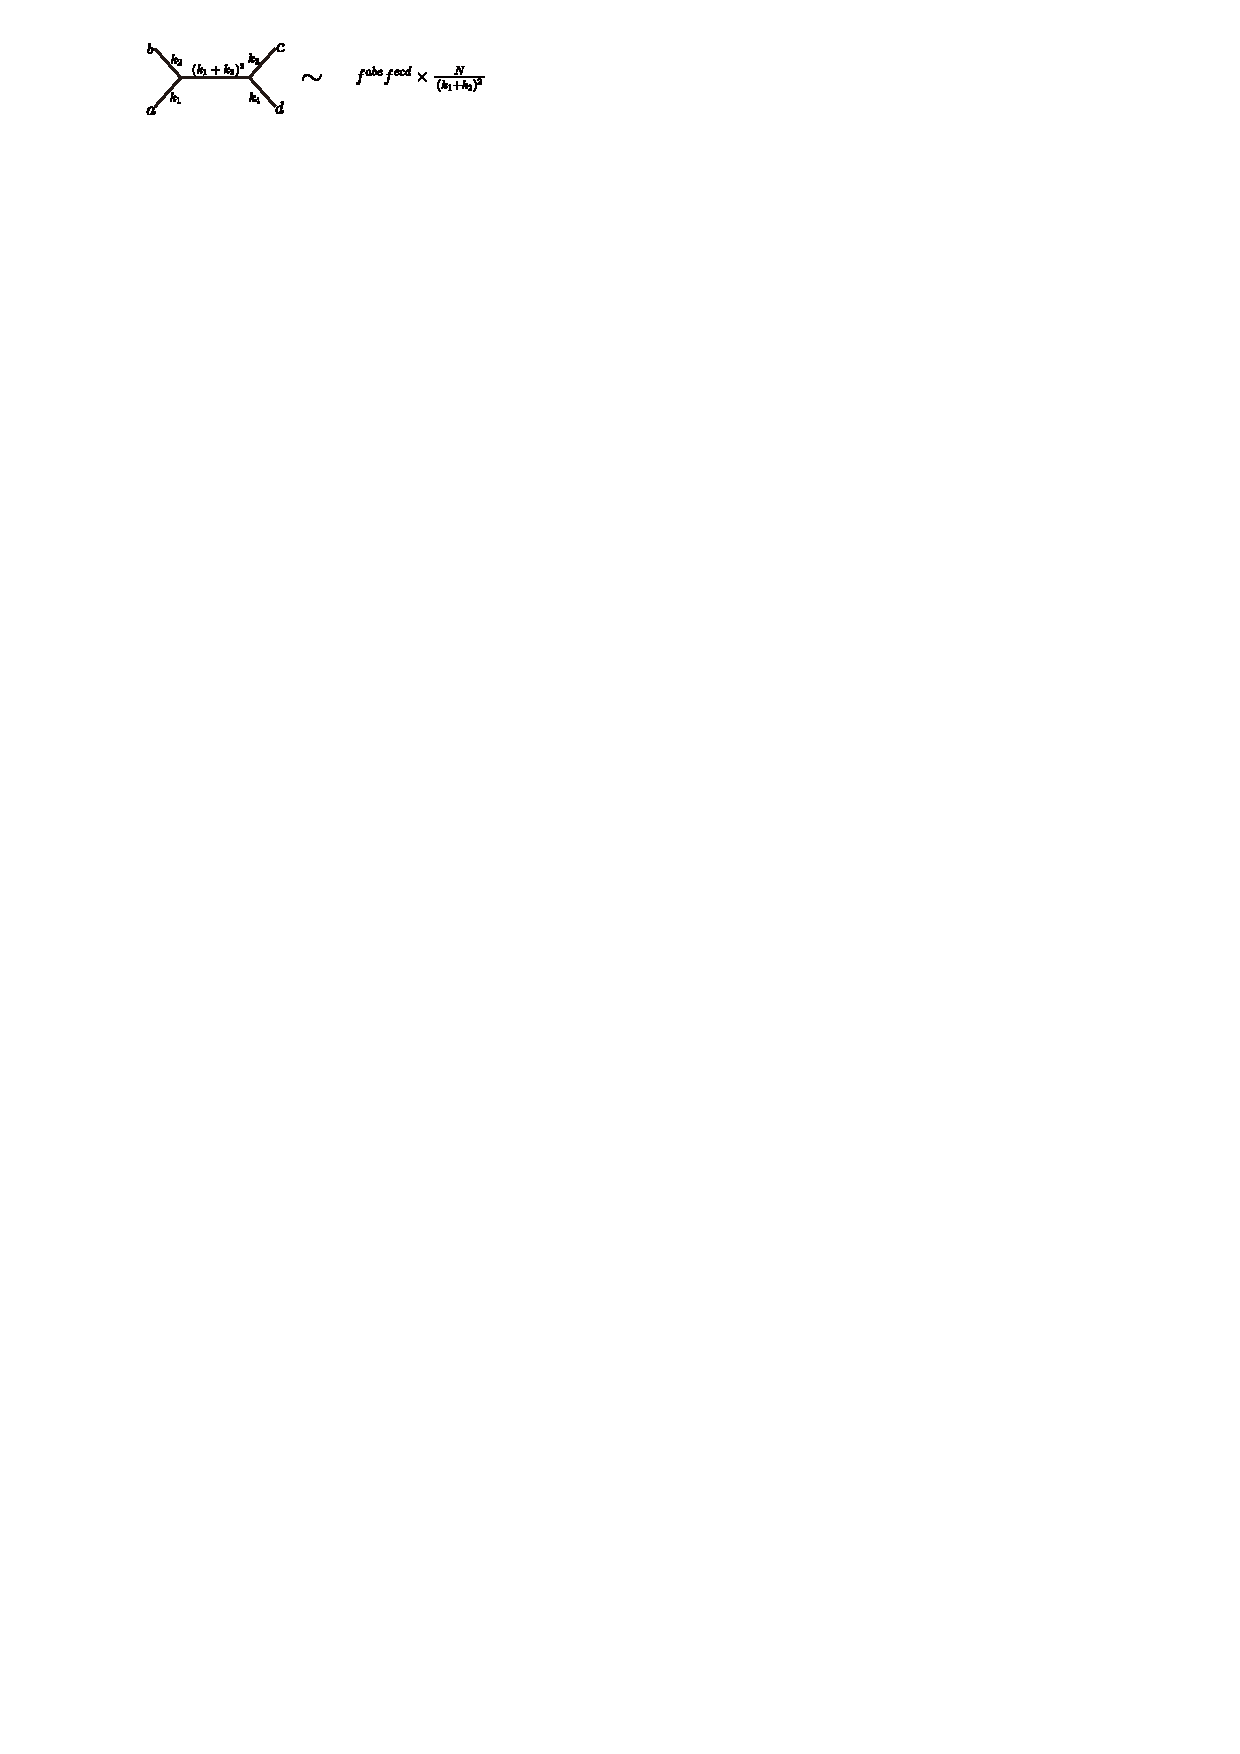
\includegraphics[width=0.8\linewidth]{figs/fig8.pdf}
	\caption{三顶点图“费曼”规则}
	\label{fig:6.1}
\end{figure}

众所周知,Yang-Mills理论费曼规则中不只有三顶角,还有四顶角,乍看之下似乎\ref{eq:6.1}有很大的漏洞。但实际上$\Gamma_n$不应该理解为费曼图,而只是组合学上对振幅的一种编码。但是这种编码的存在性又可以从费曼图本身看出来,比如费曼图四顶角可以用下面的一种方式约化为三顶角:
\begin{equation}
	\parbox[c]{\linewidth}{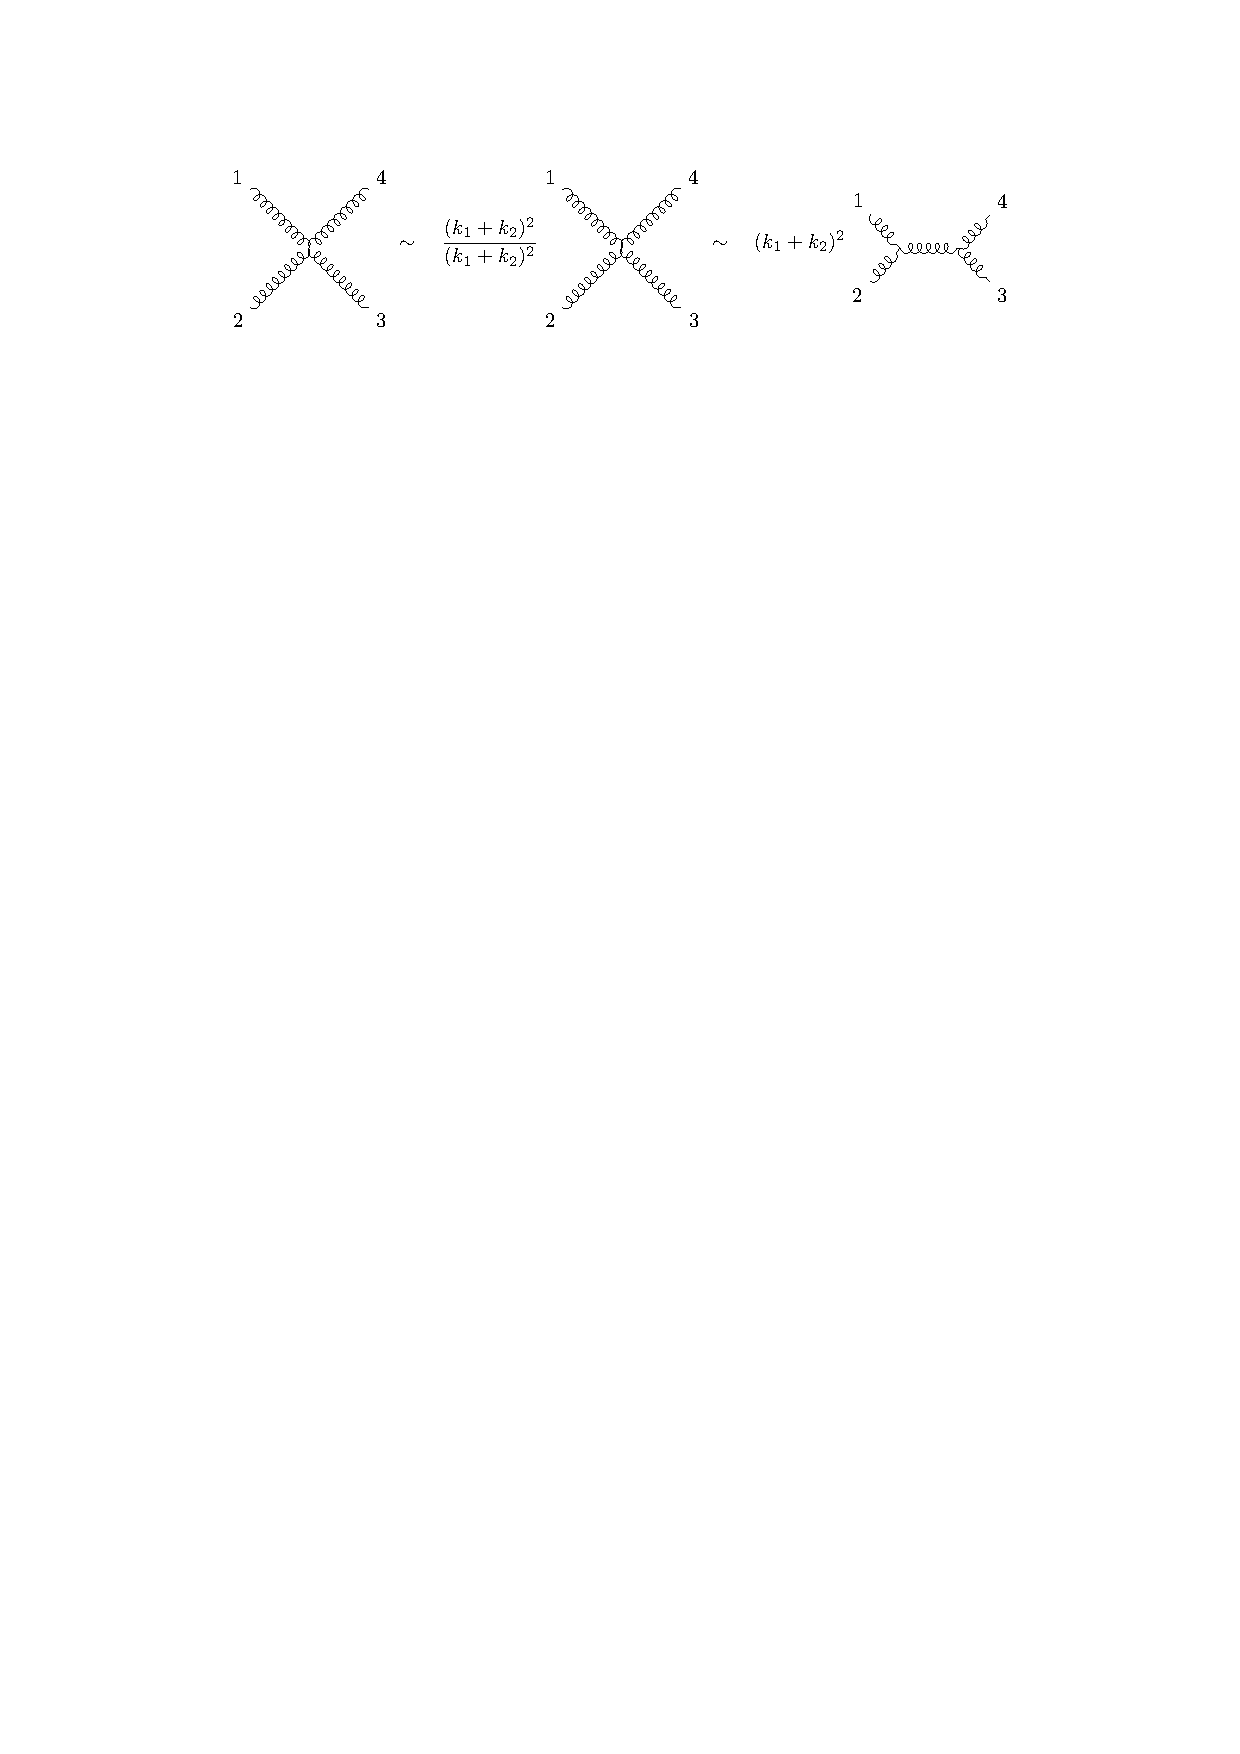
\includegraphics[width=\linewidth]{figs/eq_feyn.pdf}}
\end{equation}
显然,这种编码不是唯一的,但至少存在。结构常数满足如下的Jacobi恒等式:
\begin{equation}
	f^{abe}f^{ecd}+f^{bce}f^{ead}+f^{cae}f^{ebd}=0
\end{equation}
\begin{figure}[htbp]
	\centering
	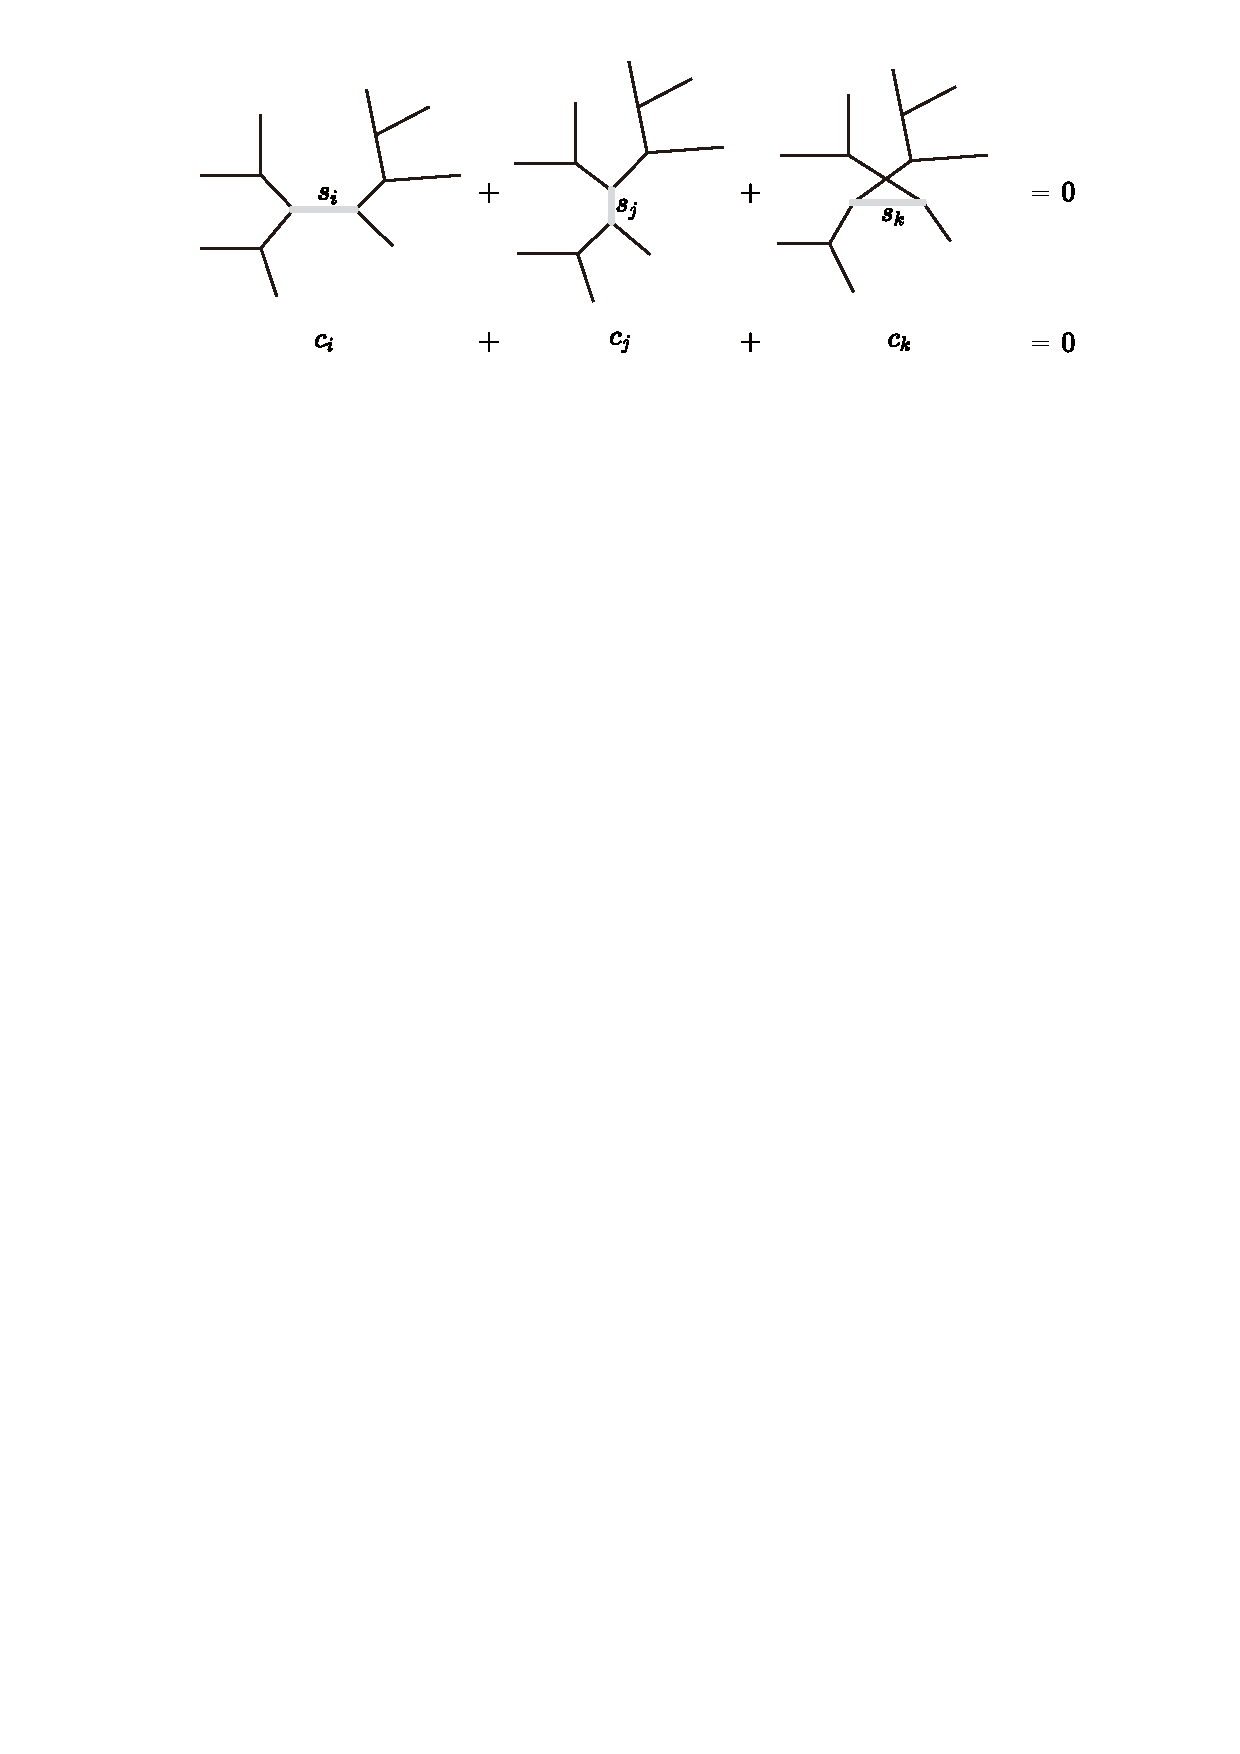
\includegraphics[width=0.95\linewidth]{figs/fig9.pdf}
	\caption{Jacobi恒等式}
	\label{fig:6.2}
\end{figure}
如图\ref{fig:6.2},这意味着三类图的色因子$c$之间的关系。同理$f^{abc}=-f^{acb}$也给出图上的关系。Bern-Carrasco-Johanson猜想存在$\{N_i\}$满足\ref{eq:6.1}而且满足和$\{c_i\}$同样的李代数结构\cite{Bern:2008qj}。也就是说对于任意$i,j,k\in\Gamma_n$:
\begin{equation}
\begin{aligned}
		c_i=-c_j\quad&\Leftrightarrow\quad N_i=-N_j\\
	c_i+c_j+c_k=0\quad&\Leftrightarrow\quad N_i+N_j+N_k=0
\end{aligned}
\end{equation}
这样的$\{N_i\}$称为BCJ分子,这个猜想也被称为色-运动学对偶。而且不难发现BCJ分子的选取不是唯一的,我们总是可以选取任意一个函数$\Delta$做如下变换得到新的BCJ分子:
\begin{equation}
	\label{eq:6.5}
	N_i\to N_i+s_i\Delta,\quad N_j\to N_j+s_j\Delta,\quad N_k\to N_k+s_k\Delta
\end{equation}
这里$s_i$,$s_j$和$s_k$是三幅图各自特有的传播子极点。对于后面要讨论的树图选取$[\lambda^a,\lambda^b] = f^{abc}\lambda^c$以及$\tr [\lambda^a,\lambda^b]=\delta^{ab}$的归一化约定,色基和迹基有如下关系:
\begin{equation}
	\label{eq:6.6}
	f^{a_1a_2x_1}f^{x_1a_3x_2}\cdots f^{x_{n-3}a_{n-1}a_n}=\operatorname{tr}\left(\lambda^{a_1}\left[\lambda^{a_2},[\lambda^{a_3},\ldots,[\lambda^{a_{n-1}},\lambda^{a_n}]\ldots]\right]\right)
\end{equation}
显然$\ref{eq:6.1}$给出如下的色序振幅:
\begin{equation}
	A_n(P)=\sum_{i\in\Gamma_n}\frac{N_i}{D_i}c_i\mid_{\tr (\lambda^P)}
\end{equation}
其中$c_i\mid_{\tr (\lambda^P)}\in\{0,\pm1\}$表示$c_i$中$\tr (\lambda^P)$前的符号。在后面对树图的讨论中,Del Duca–Dixon–Maltoni 基底是十分有用的\footnote{DelDuca:1999rs}:
\begin{equation}
	\label{eq:6.9}
	\mathcal{A}_n = \sum_{\sigma \in S_{n-2}} f^{a_1 a_{\sigma_1} b_1} f^{b_1 a_{\sigma_2} b_2} \cdots f^{b_{n-3} a_{\sigma_{n-2}} a_n} A_n(1, \sigma_1, \sigma_2, \ldots, \sigma_{n-2}, n)
\end{equation}
原本色运动学分离给出迹基底下的展开:
\begin{equation}
	\label{eq:6.10}
	\mathcal{A}_n=\sum_{\sigma\in S_{n-1}}\tr (\lambda^{a_{\sigma_1}}\lambda^{a_{\sigma_2}}\cdots \lambda^{a_{\sigma_{n-1}}}\lambda^{a_n})A_n(\sigma_1,\sigma_2,\ldots,\sigma_{n-1},n)
\end{equation}
但这些色序振幅之间仍有K-K关系\ref{KK},另外色基和迹基之间有关系\ref{eq:6.6},联合起来便可以从\ref{eq:6.10}转换到\ref{eq:6.9}。DDM基底的那些色因子之间是雅可比恒等式意义下独立的,他们对应半梯子图\ref{fig:6.3},后面记其色因子为$c_{1|\sigma|n}$。由于Jacobi恒等式,总可以将\ref{eq:6.1}利用图\ref{fig:6.4}的过程转换成\ref{eq:6.9}的形式。也就是说半梯子图是$\Gamma_n$中的一组独立基底,在构造BCJ分子是我们并不需要半梯子图的$\{N_i\}$之间满足Jacobi恒等式,利用半梯子图用Jacobi恒等式构造剩下的BCJ分子,然后要求求和后刚好得到规范理论振幅。
\begin{figure}[htbp]
	\centering
	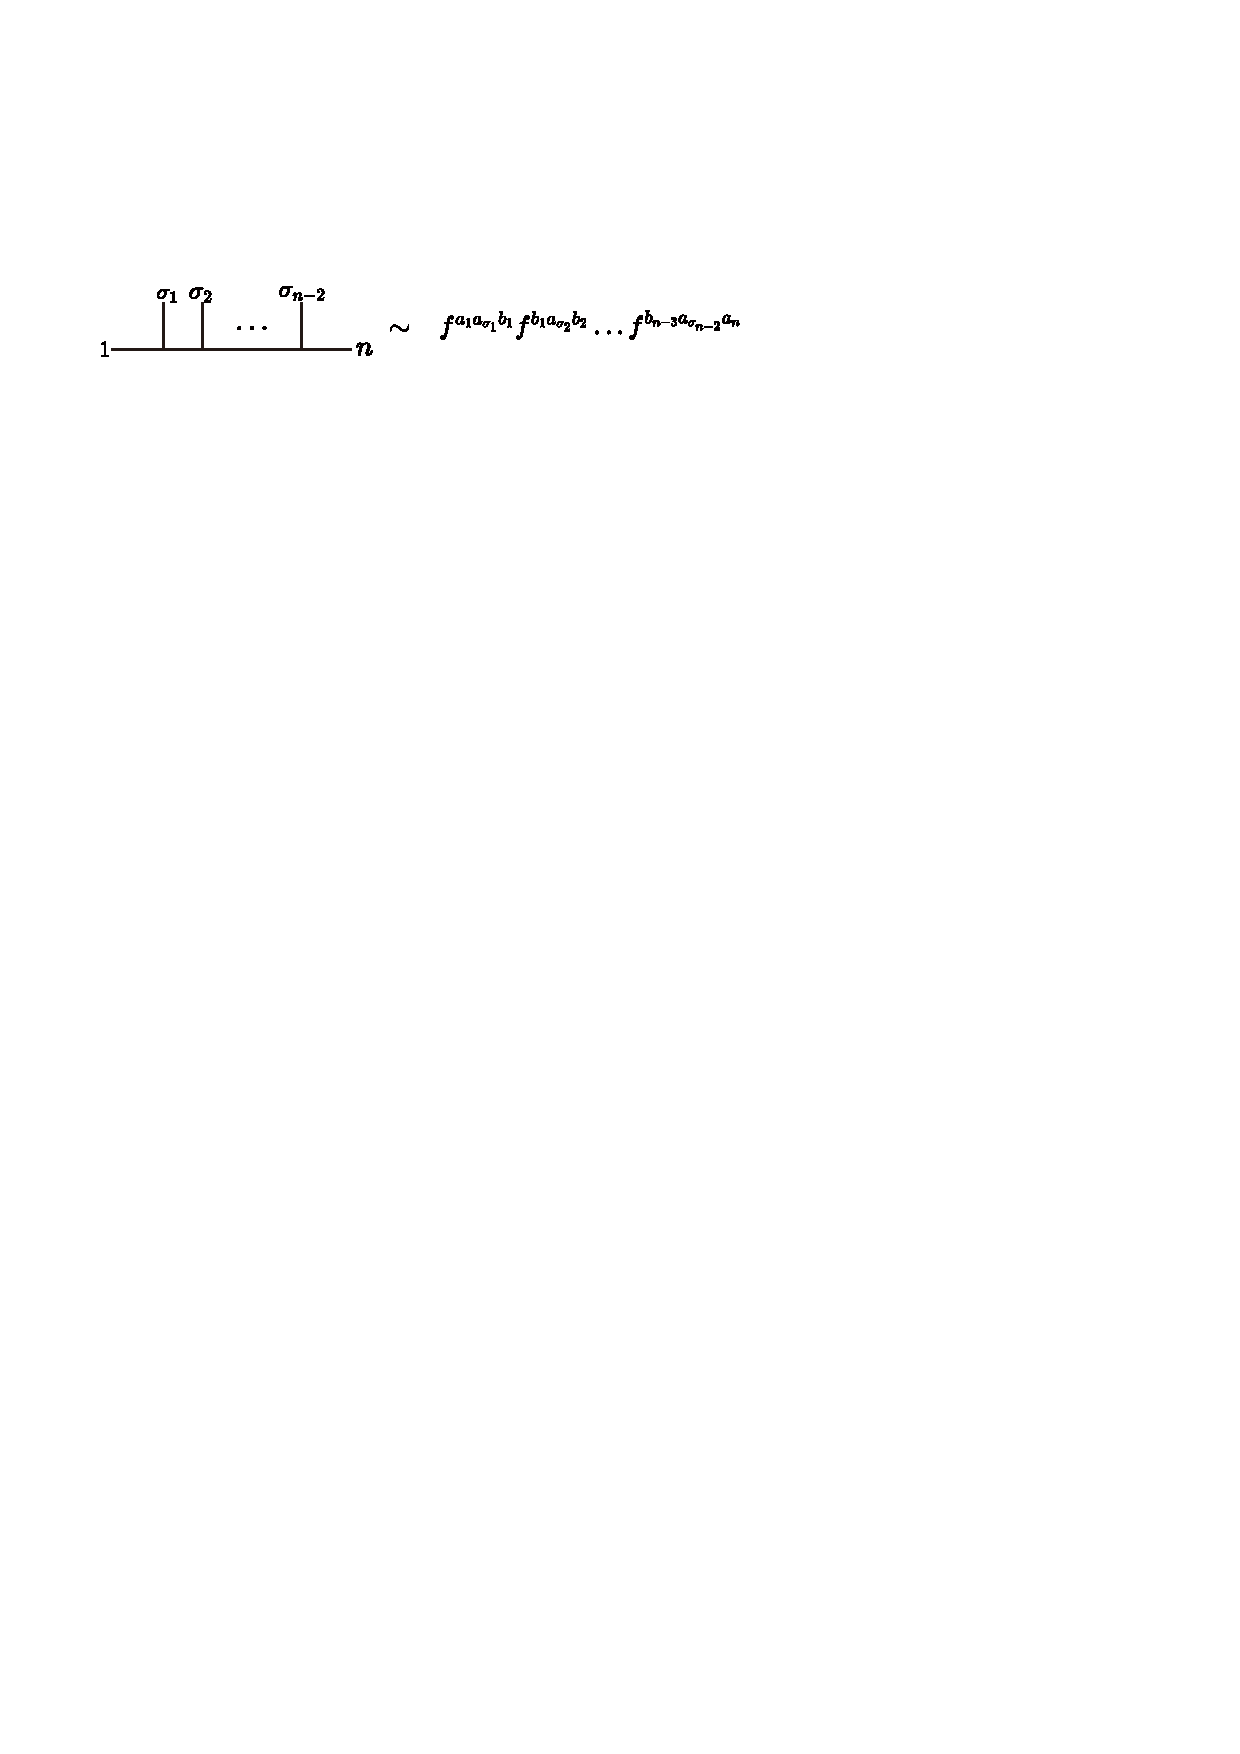
\includegraphics[width=0.95\linewidth]{figs/fig10.pdf}
	\caption{半梯子图}
	\label{fig:6.3}
\end{figure}

\begin{figure}[htbp]
	\centering
	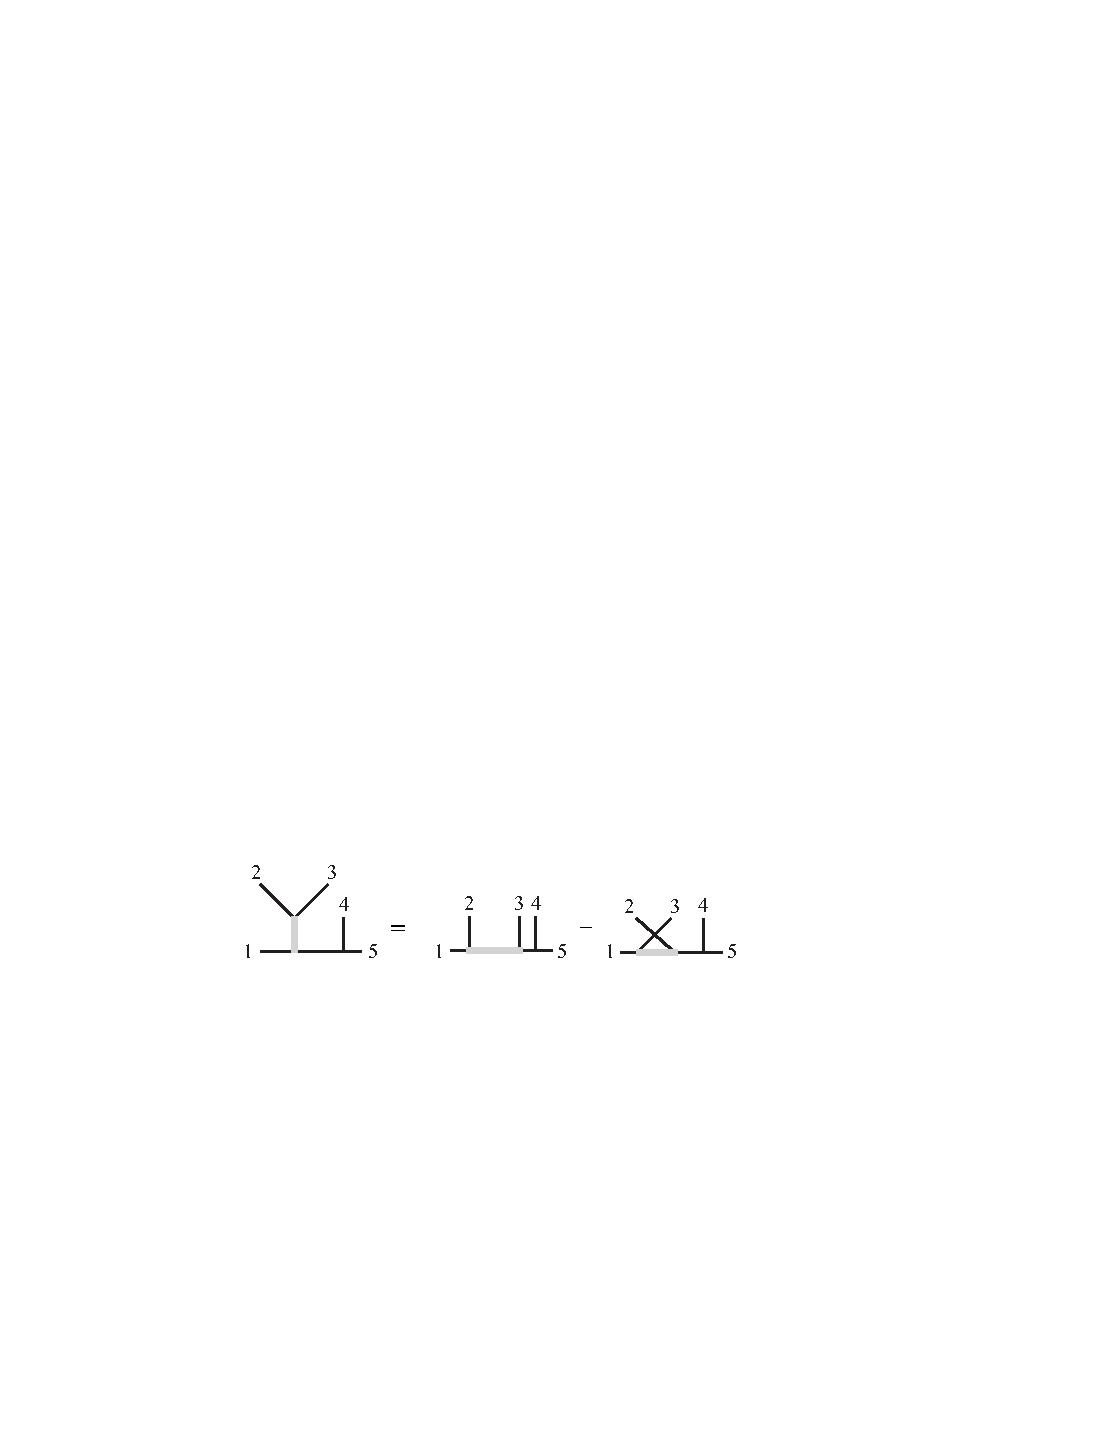
\includegraphics[width=0.90\linewidth]{figs/fig11.pdf}
	\caption{利用Jacobi恒等式转换到半梯子图}
	\label{fig:6.4}
\end{figure}

\begin{figure}[htbp]
	\centering
	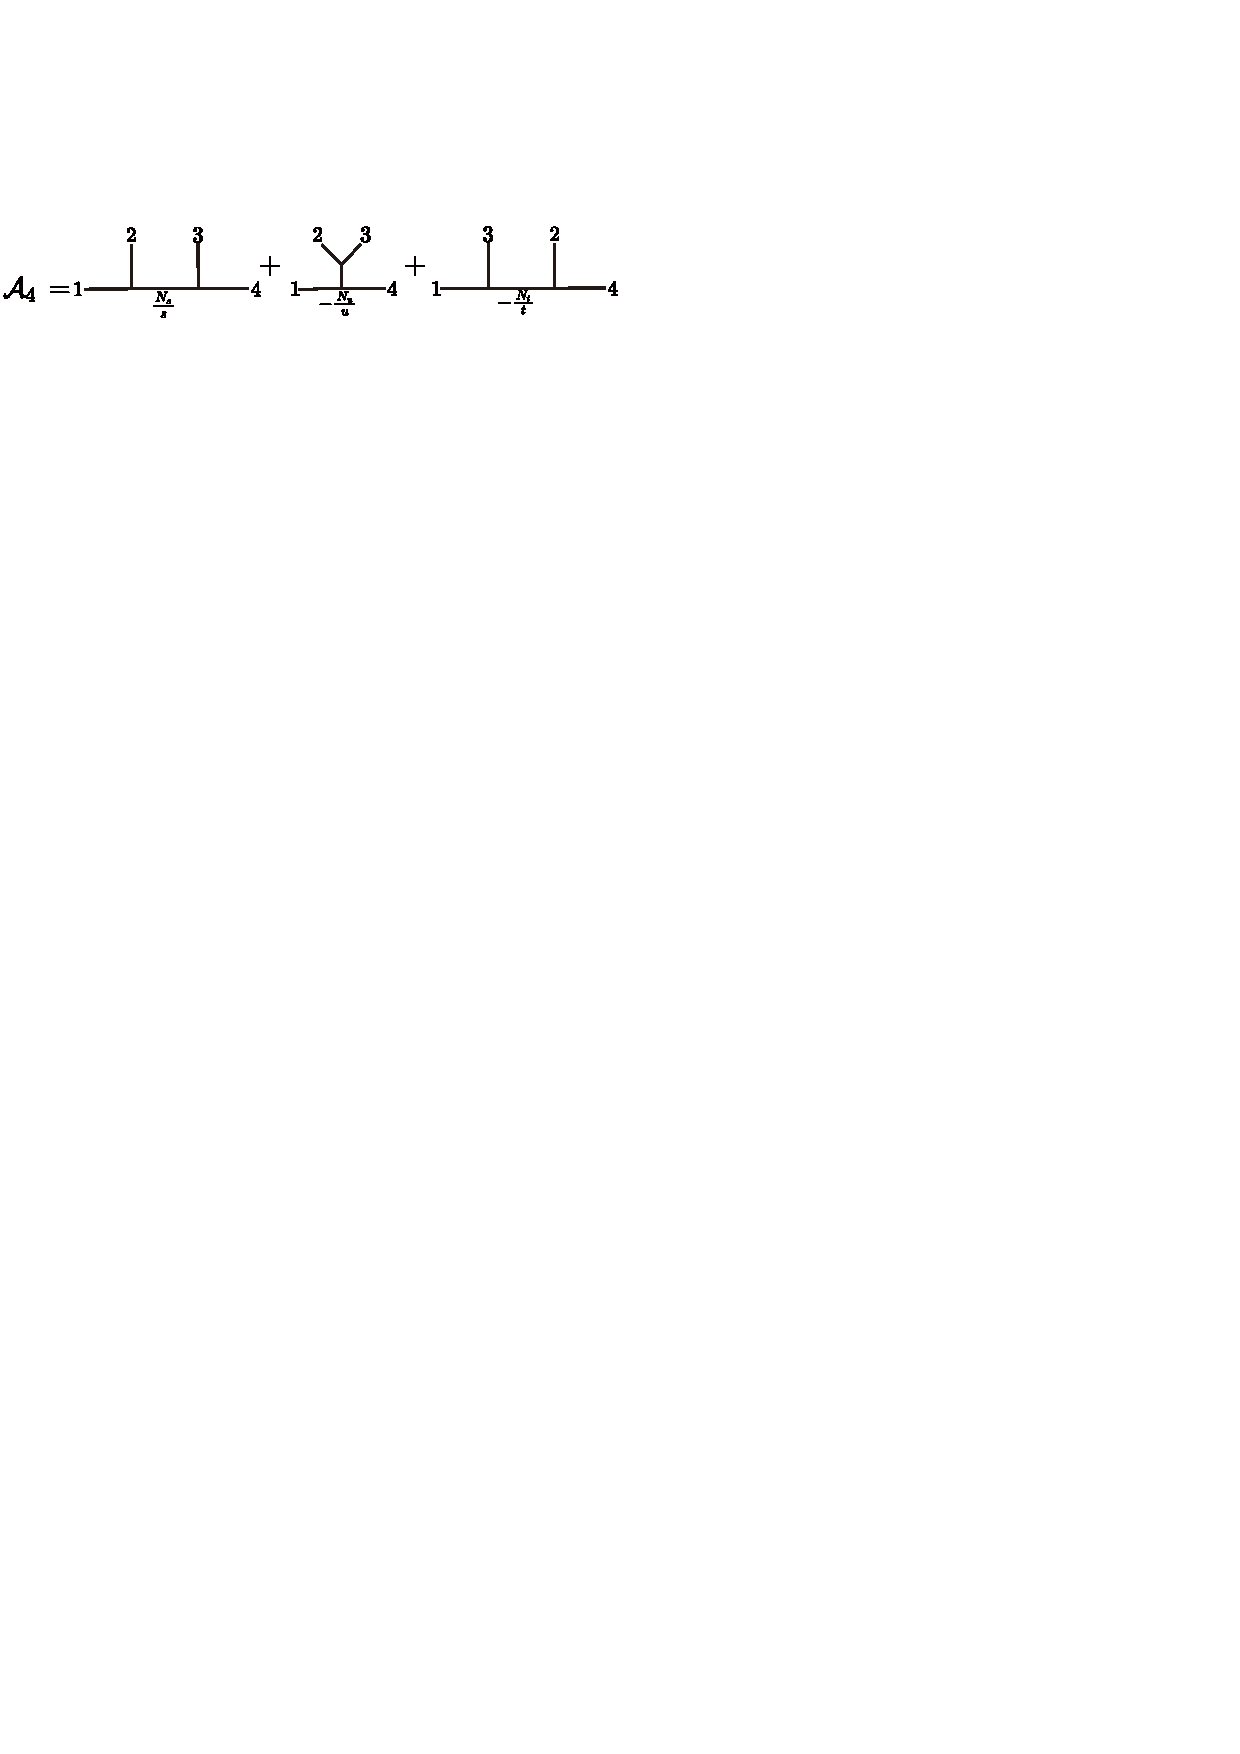
\includegraphics[width=0.90\linewidth]{figs/fig12.pdf}
	\caption{$\Gamma_4$的三幅图}
	\label{fig:6.5}
\end{figure}
比如四点Yang-Mills理论振幅有\ref{fig:6.5}三幅三顶角图有贡献。这里选取正负号约定是为了让$N_s+N_u+N_t=0$,对于树图$m$点情况$|\Gamma_m|=(2m-5)!!$。四点情况下只有两个偏振幅在Jacobi等式的意义下线性独立\footnote{当然如果加入BCJ恒等式两者也线性相关。},选取固定$1$和$4$。将\ref{fig:6.5}中第二个图利用Jacobi恒等式展开到半梯子图得到:
\begin{equation}
	A(1234) = \frac{N_s}{s}-\frac{N_u}{u},\quad A_4(1324)=-\frac{N_t}{t}+\frac{N_u}{u}
\end{equation}
不难看出上面偏振幅在\ref{eq:6.5}的变换下是规范不变的,其实就是在说单个三顶角图不是可观测量,但组合在一起得到的偏振幅规范不变。而且从$N_s+N_t+N_u=0$导出他们满足BCJ恒等式$sA_4(1,2,3,4)=tA_4(1,3,2,4)$。注意,如果$\{N_i\}$是BCJ分子,那么BCJ恒等式自然被满足,但BCJ恒等式本身是和\ref{eq:6.1}的参数化选取无关的,也就是说不管$\{N_i\}$如何选取,最终的振幅之间都满足BCJ恒等式。选取$N_s$和$N_u$为独立变量:
\begin{equation}
	\begin{pmatrix}A_4(1234)\\A_4(1324)\end{pmatrix}=\begin{pmatrix}\frac{1}{s}&-\frac{1}{u}\\\frac{1}{t}&\frac{1}{u}+\frac{1}{t}\end{pmatrix}\begin{pmatrix}N_s\\N_u\end{pmatrix}
\end{equation}
但是由于偏振幅之间满足BCJ恒等式,他们之间不是线性无关的,所以上面的矩阵其实不可逆。而这又恰恰说明了BCJ分子的不唯一性。

上面说的这些都仅仅只是色-运动学之间代数结构上的对偶,而这种对偶和规范理论与微扰引力理论振幅之间又密切关系。进一步有猜想,如果找到了一组BCJ分子,那么引力振幅可以直接由\ref{eq:6.1}得到:
\begin{equation}
	\mathcal{M}_n=\sum_{i\in\Gamma_n}\frac{N_iN_i}{D_i}=\sum_{i\in\Gamma_n}\frac{N_i\tilde{N}_i}{D_i}
\end{equation}
此式称为BCJ双复制关系。第二个等号是说明双复制的$n_i$可以只有一个是BCJ分子,另外一个可以不满足色运动学对偶,但是最终得到的振幅依然相同。利用半梯子图基底可以写成下式:
\begin{equation}
	\label{eq:6.14}
	M_n=\sum_{\sigma\in S_{n-2}}n_{1|\sigma_1,\sigma_2,\ldots,\sigma_{n-2}|n}A_n(1,\sigma_1,\sigma_2,\ldots,\sigma_{n-2},n)
\end{equation}
所以只需要知道半梯子图的BCJ分子就够了。前面我们讲过KLT关系,也是双复制的形式。实际上KLT关系可以看作是树图的一组特殊的BCJ双复制关系,可以从KLT关系直接构造出半梯子图的BCJ分子从而用Jacobi恒等式得到三顶点图的全部BCJ分子,比如四点五点KLT关系为:
\begin{equation}
\begin{aligned}
	M_4(1234)&=-s_{12}A_4(1234)A_4(1243),\\M_5(12345)&=s_{23}s_{45}A_5(12345)A_5(13254)+(3\leftrightarrow4)
\end{aligned}
\end{equation}
与\ref{eq:6.14}对照可以得到BCJ分子:
\begin{equation}
	\begin{aligned}
		n=4:\quad & n_{12,34} = -s_{12}\,A^{\text{tree}}_{4}[1243], \quad n_{13,24} = 0; \\
		n=5:\quad & n_{12,3,45} = s_{23}\,s_{45}\,A^{\text{tree}}_{5}[13254], \quad n_{12,4,35} = s_{24}\,s_{35}\,A^{\text{tree}}_{5}[14253]; \\
		& n_{13,4,25} = n_{14,2,35} = n_{14,3,215} = n_{12,3,415} = 0.
	\end{aligned}
\end{equation}
树图的BCJ双复制关系已经得到证明\cite{Bern:2010yg},但目前对于圈图BCJ分子的构造仍是一个未解之谜,不过已经构造出了不少例子\cite{Bern:2010ue,Bern:2012uf},这也让我们相信色-运动学对偶猜想的正确性。近年来,双复制关系也被用在引力波求解等问题上,详见综述\cite{Bern:2019prr,Adamo:2022dcm,Bern:2022wqg}。

\section{纯旋量超弦关联函数计算}
纯旋量形式计算涉及到OPE计算以及展开超场后计算鬼场零模,本章我们不去关注后面一部分,而关注如何计算OPE。从$\S$\ref{sec:5.4}可以看出如果直接使用$\partial\theta$,$\Pi$,$d$,$N$的OPE计算会非常复杂,我们试图把顶角算符本身作为一个整体来计算OPE,比如:
\begin{equation}
	V_1(z_1)V_2(z_2)\sim 0
\end{equation}
\begin{equation}
	\label{eq:6.17}
	V_1(z_1)U_2(z_2)\sim z_{12}^{-k_1\cdot k_2}\frac{L_{12}(z_2)}{z_{12}},\quad L_{12}:=-A_2^m(\lambda\gamma_mW_1)-V_2(k_2\cdot A_1)+Q(A_2W_1)
\end{equation}
\begin{equation}
	\label{eq:6.18}
	\begin{aligned}
		U_1(z_1)U_2&(z_2)\sim z_{12}^{-k_1\cdot k_2-1}\left(\partial\theta^\alpha\Big[(k_1\cdot A_2)A_\alpha^1-(k_2\cdot A_1)A_\alpha^2+D_\alpha A_\beta^2W_1^\beta-D_\alpha A_\beta^1W_2^\beta\Big]\right.\\&+\Pi^m\Big[(k_1\cdot A_2)A_m^1-(k_2\cdot A_1)A_m^2+k_m^2(A_2W_1)-k_m^1(A_1W_2)-(W_1\gamma_mW_2)\\&+d_\alpha\left[(k_1\cdot A_2)W_1^\alpha-(k_2\cdot A_1)W_2^\alpha+\frac14(\gamma^{mn}W_1)^\alpha F_{mn}^2-\frac14(\gamma^{mn}W_2)^\alpha F_{mn}^1\right]\\&+\frac12N^{mn}\Big[(k_1\cdot A_2)F_{mn}^1-(k_2\cdot A_1)F_{mn}^2-2k_m^{12}(W_1\gamma_nW_2)+2F_{ma}^1F_{na}^2\Big]\Big)\\&+(1+k_1\cdot k_2)z_{12}^{-k_1\cdot k_2-2}\left[(A_1W_2)+(A_2W_1)-(A_1\cdot A_2)\right]
	\end{aligned}
\end{equation}
其中$Q$是BRST荷,利用$d_\alpha$和超场的OPE,后面的计算可以将$Q$看作是$\lambda^\alpha D_\alpha$。计算中涉及到对超场求导,而平面波求导会出现$ik$因子,为了避免频繁出现虚数单位,我们选取约定$ik\to k$,从而Mandelstam变量与惯用的也相差$-1$。另外,我们隐藏$A^\mu$和$A_\alpha$指标,用$\cdot$表示矢量指标求和,旋量指标求和则不加任何标记。而且假设所有的超场都是$K(\theta)$,已经分离平面波。乍看之下似乎看不出规律,但倘若定义:
\begin{equation}
	\label{eq:6.19}
	\begin{aligned}
		&A_\alpha^{12}=\frac{1}{2}\left[A_\alpha^2(k_2\cdot A_1)+A_2^m(\gamma_mW_1)_\alpha-(1\leftrightarrow2)\right]
		\\&A_{12}^m=\frac{1}{2}\left[A_2^m(k_2\cdot A_1)+A_p^1F_2^{pm}+(W_1\gamma^mW_2)-(1\leftrightarrow2)\right]
		\\&W_{12}^{\alpha}=\frac{1}{4}(\gamma_{mn}W_2)^\alpha F_1^{mn}+W_2^\alpha(k_2\cdot A_1)-(1\leftrightarrow2)
		\\&F_{12}^{mn}=F_2^{mn}(k_2\cdot A_1)+\frac{1}{2}F_2^{[m}F_1^{n]p}+k_1^{[m}(W_1\gamma^{n]}W_2)-(1\leftrightarrow2)
	\end{aligned}
\end{equation}
\ref{eq:6.18}变成:
\begin{equation}
	\label{eq:6.20}
	\begin{aligned}
		&U_1(z_1)U_2(z_2)\sim-z_{12}^{-k_1\cdot k_2-1}\left(\partial\theta^\alpha A_\alpha^{12}+\Pi^mA_m^{12}+d_\alpha W_{12}^\alpha+\frac{1}{2}N^{mn}F_{mn}^{12}\right)\\&+\partial_1\left(z_{12}^{-k_1\cdot k_2-1}\left[\frac{1}{2}(A_1\cdot A_2)-(A_1W_2)\right]\right)-\partial_2\left(z_{12}^{-k_1\cdot k_2-1}\left[\frac{1}{2}(A_1\cdot A_2)-(A_2W_1)\right]\right)
	\end{aligned}
\end{equation}
注意到$U$是积分顶角算符,可以预料到这些全导数项应当能够忽略,得到下面的等效OPE:\footnote{\ref{eq:6.20}中的$z_{12}^{-k_1\cdot k_2}$因子来源于平面波给出的Koba-Nielsen因子,注意这里我们已经假设所有的超场都是不带平面波因子的,这从运动方程就能看出来这一约定。最后计算振幅只需要补上Koba-Nielsen因子即可。}\footnote{似乎在OPE之后还会剩下$\partial\theta,\Pi,\ldots$,并非超场零模积分,但注意到盘面振幅始终存在无积分顶角算符插入,所以最终振幅一定可以用$\langle V_P\rangle$表示。}
\begin{equation}
	U_1(z_1)U_2(z_2)\cong \frac{U_{12}(z_2)}{z_{12}}, \quad U_{12}:=\partial\theta^\alpha A_\alpha^{12}+\Pi^mA_m^{12}+d_\alpha W_{12}^\alpha+\frac{1}{2}N^{mn}F_{mn}^{12}
\end{equation}
同理,注意到下式BRST恰当:
\begin{equation}
	L_{21}+L_{12}=Q\left[(A_1W_2)+(A_2W_1)-(A_1\cdot A_2)\right]
\end{equation}
所以$L_{12}$的对称部分应当和体系解耦,利用\ref{eq:6.17}以及\ref{eq:6.19}不难验算在去除掉所有BRST恰当的项之后有如下等效OPE:
\begin{equation}
	V_1(z_1)U_2(z_2)\cong \frac{V_{12}(z_2)}{z_{12}},\quad
	V_{12} := \lambda^\alpha A_\alpha^{12}
\end{equation}
代入\ref{eq:5.45}得到新定义的包含多个指标的超场(多粒子超场)满足:
\begin{equation}
	\begin{aligned}
		D_\alpha A_\beta^{12}+D_\beta A_\alpha^{12}&=\gamma_{\alpha\beta}^mA_m^{12}{\color{blue}+(k_1\cdot k_2)(A_\alpha^1A_\beta^2+A_\beta^1A_\alpha^2)}
		\\D_\alpha A_{12}^m&=\gamma_{\alpha\beta}^mW_{12}^\beta{+\color{blue}k_{12}^mA_\alpha^{12}+(k_1\cdot k_2)(A_\alpha^1A_2^m-A_\alpha^2A_1^m)}
		\\D_\alpha W_{12}^\beta&=\frac{1}{4}(\gamma_{mn})_\alpha^\beta F_{12}^{mn}{\color{blue}+(k_1\cdot k_2)(A_\alpha^1W_2^\beta-A_\alpha^2W_1^\beta)}
		\\D_\alpha F_{12}^{mn}&=k_{12}^{[m}(\gamma^{n]}W_{12})_\alpha{\color{blue}+(k_1\cdot k_2)\left[A_\alpha^1F_2^{mn}+A_1^{[n}(\gamma^{m]})W_2)_\alpha-(1\leftrightarrow2)\right]}
	\end{aligned}
\end{equation}
\begin{equation}
	F_{12}^{mn}=k_{12}^mA_{12}^n-k_{12}^nA_{12}^m{\color{blue}-(k_1\cdot k_2)(A_1^mA_2^n-A_1^nA_2^m)}
\end{equation}
不难发现相比于\ref{eq:5.45}多了蓝色标出的“接触项”,同样的,多粒子顶角算符也会多出一些接触项,而不是简单的BRST闭:
\begin{equation}
	\label{eq:6.26}
	\begin{aligned}
		QV_{12}&={\color{blue}(k_1\cdot k_2)V_1V_2}\\
		QU_{12}&=\partial V_{12}{\color{blue}+(k_1\cdot k_2)(V_1U_2-V_2U_1)}
	\end{aligned}
\end{equation}
但倘若我们能找到接触项的一般表达式,解相应的场方程找到多粒子超场类似单粒子超场的$\theta$展开,那么我们就能利用OPE的规律很快解决振幅计算问题。Mafra和Schlotterer正是利用这一点得到了超弦无质量态$n$点盘面振幅的一般公式\cite{Mafra:2011nv,Mafra:2011nw},接下来我们先来研究一般的多粒子超场。
\subsection{多粒子超场}
前面两个顶角算符的缩并我们改为使用$V_{[1,2]}$表示,不难发现$V_{12} = -V_{21}$确实有李括号带来的反对易性。类似的,还会有多个缩并,比如$U_1(z_1)U_2(z_2)U_3(z_3)$:
\begin{equation}
	U_{[[1,2],3]}(z_3),\quad U_{[1,[2,3]]}(z_3),\quad U_{[1,[2,3]]}(z_3)
\end{equation}
这种下标称为李多项式\footnote{之后大写字母$P,Q,\ldots$表示李多项式或者字词,从上下文不至于混淆。},数学方面的介绍可见\cite{REUTENAUER2003887, free_lie,lothaire1997combinatorics},更偏向物理的介绍可见\cite{Frost:2020eoa}。使用这种下标的好处是显现出了最终我们得到的多粒子超场/顶角算符关于指标的对称性,后面我们会尽可能构造超场使得其拥有李多项式所满足的对称性,这是本文后面用于构建BCJ分子的核心。现在我们期望多个顶角算符缩并得到的$U_\Gamma$和$V_{\Gamma}$仍像上一节一样可以通过定义对应的$A^\Gamma$,$W^\Gamma$和$F^\Gamma$得到类似顶角算符的形式。后面定义多粒子超场都是在李多项式的意义下定义的,对下指标做线性扩张便可得到对字词定义的多粒子超场。比如$V_{12}$\footnote{不要与上一小节中的$V_{12}$弄混。}就是$V_{[1,2]}$的对称部分。

由于多粒子超场本身来源于单粒子超场,而单粒子超场本身是离壳的,也就是说存在规范对称性。比如展开单粒子超场时就使用的是Harnad–Shnider规范。所以多粒子场本身也应当有这种规范选取带来的不唯一性,下面逐一讨论。
\subsubsection{Lorenz规范}
最早在Lorenz规范$\partial\cdot A^P = 0 $下找到了多粒子超场满足的递推公式:
\begin{equation}
	\begin{aligned}
	\hat{A}_\alpha^{[P,Q]}&=\frac{1}{2}\left[\hat{A}_\alpha^Q(k_Q\cdot\hat{A}_P)+\hat{A}Q^m(\gamma_m\hat{W}_P)\alpha-(P\leftrightarrow Q)\right]\\
	\hat{A}_{[P,Q]}^m&=\frac{1}{2}\left[\hat{A}_Q^m(k_Q\cdot\hat{A}_P)+\hat{A}_n^P\hat{F}_Q^{nm}+(\hat{W}_P\gamma^m\hat{W}_Q)-(P\leftrightarrow Q)\right]\\
	\hat{W}_{[P,Q]}^{\alpha}&=\frac{1}{4}\hat{F}_P^{rs}(\gamma_{rs}\hat{W}_Q)^\alpha+\frac{1}{2}(k_Q\cdot\hat{A}_P)\hat{W}_Q^\alpha+\frac{1}{2}\hat{W}_Q^{m\alpha}\hat{A}_m^P-(P\leftrightarrow Q)\\
	\hat{F}_{[P,Q]}^{mn}&=\frac{1}{2}{\left[\hat{F}_Q^{mn}(k_Q\cdot\hat{A}_P)+\hat{F}_Q^{p|mn}\hat{A}_p^p+\hat{F}_Q^{[m}\hat{F}_P^{n]r}-2\gamma_{\alpha\beta}^{[m}\hat{W}_P^{n]\alpha}\hat{W}_Q^\beta-(P\leftrightarrow Q)\right]}
\end{aligned}
\end{equation}
递推初始项来源于$\hat K_i = K_i$,动量应当理解为无视李括号,比如$k_{[1,[2,3]]}:=k_{123}:=\sum_{i=1}^3k_i$。其中:
\begin{equation}
\begin{aligned}
		\hat{W}_{[P,Q]}^{m\alpha} &= k_{PQ}^m \hat{W}_{[P,Q]}^\alpha - (\hat{A}^m \otimes \hat{W}^\alpha)_{C([P,Q])} \\
	\hat{F}_{[P,Q]}^{m|pq} &= k_{PQ}^m \hat{F}_{[P,Q]}^{pq} - (\hat{A}^m \otimes \hat{F}^{pq})_{C([P,Q])}
\end{aligned}
\end{equation}
这里我们引入了接触项算符$C$,递归定义为,$C(i):= 0 $:
\begin{equation}
	C([P,Q]):=[C(P),Q]+[P,C(Q)]+(k_P\cdot k_Q)(P\otimes Q-Q\otimes P)
\end{equation}
张量积满足莱布尼茨律:
\begin{equation}
\begin{aligned}
		[A\otimes B,Q]:=[A,Q]\otimes B+A\otimes[B,Q]\\
	[P,A\otimes B]:=[P,A]\otimes B+A\otimes[P,B]
\end{aligned}
\end{equation}
后面还会用到反对易楔积的定义:
\begin{equation}
	P\wedge Q:=P\otimes Q-Q\otimes P
\end{equation}
且依照线性扩张定义:
\begin{equation}
	(K\otimes T)_{P\otimes Q}:=K_PT_Q,\quad(K\wedge T)_{P\wedge Q}:=K_PT_Q
\end{equation}
把$C$称为接触项算符是有原因的,超场运动方程的接触项恰好是由$C[P,Q]$生成的:
\begin{equation}
\begin{aligned}
	D_{(\alpha}\hat{A}_{\beta)}^{[P,Q]}&=\gamma_{\alpha\beta}^m\hat{A}_m^{[P, {Q}]}{\color{blue}+(\hat{A}_\alpha\otimes\hat{A}_\beta)_{ {C}([P, {Q}])}}
	\\D_\alpha\hat{A}_m^{[P,Q]}&=(\gamma_m\hat{W}^{[P, {Q}]})_\alpha+k_m^{ {PQ}}\hat{A}_\alpha^{[P, {Q}]}{\color{blue}+(\hat{A}_\alpha\otimes\hat{A}^m)_{ {C}([P, {Q}])}}
	\\D_\alpha\hat{W}_{[P, {Q}]}^\beta&=\frac{1}{4}(\gamma^{mn})_\alpha^\beta\hat{F}_{mn}^{[P,Q]}{\color{blue}+(\hat{A}_\alpha\otimes\hat{W}^\beta)_{C([P,Q])}}
	\\D_\alpha\hat{F}_{[P,Q]}&=\left(\hat{W}_{[P,Q]}^{[m}\gamma^{n]}\right)_\alpha{\color{blue}+(\hat{A}_\alpha\otimes\hat{F}^{mn})_{ {C}([P,Q])}}
\end{aligned}
\end{equation}
\begin{equation}
	\label{eq:6.35}
	\hat{F}_{[P,Q]}^{mn}=k_{PQ}^m\hat{A}_{[P,Q]}^n-k_{PQ}^m\hat{A}_{[P,Q]}^m{\color{blue}-(\hat{A}^m\otimes\hat{A}^n)_{C([P,Q])}}
\end{equation}
\subsubsection{混合(hybrid)规范}
Dynkin括号递归定义为:
\begin{equation}
	\ell(123\ldots n):=[\ell(123\ldots n-1),n]
\end{equation}
其满足下面的Baker恒等式:
\begin{equation}
	\ell(P\ell(Q))=[\ell(P),\ell(Q)]
\end{equation}
显然$A\ell(B)+B\ell(A)\in\ker\ell$,而且由$\ell$的递归定义知$\forall Q$,$\ell(P) = 0\Rightarrow \ell(PQ)=0$。前面说过我们希望多粒子超场的定义尽可能展现出李多项式本身的对称性,那么如果$K\approx \ell$,也就是说满足下面的广义BCJ恒等式:
\begin{equation}
	\label{eq:6.38}
	K_{A\ell(B)C}+K_{B\ell(A)C}=0,\quad A,B\neq\varnothing,\quad\forall C
\end{equation}
当$B=i$时上式简化为BCJ恒等式:
\begin{equation}
	\label{eq:6.39}
	K_{AiB}=-K_{i\ell(A)B},\quad A\neq\emptyset,\forall B
\end{equation}
这其实就是$K_P\leftrightarrow c_P$的“色-运动学”对偶下要求$K_P$也满足Jacobi恒等式。这样的超场被称作处在BCJ规范的超场,不加任何符号以区分Lorenz等规范下超场。本节要介绍的混合规范本身并不是计算上会用到的规范,更应该看作是为了构造BCJ规范超场的一种定义:
\begin{equation}
	\begin{aligned}
		\check{A}_\alpha^{[P,  {Q}]}&=\frac{1}{2}[A_\alpha^  {Q}(k_Q\cdot A_P)+A_Q^m(\gamma_mW_P)_\alpha-(P\leftrightarrow Q)]
		\\\check{A}_{[P,  {Q}]}^m&=\frac{1}{2}[A_Q^m(k_Q\cdot A_P)+A_n^PF_Q^{nm}+(W_P\gamma^mW_Q)-(P\leftrightarrow Q)]\\
		\check{W}_{[P,  {Q}]}^\alpha&=\frac{1}{4}F_P^{rs}(\gamma_{rs}W_Q)^\alpha+\frac{1}{2}(k_Q\cdot A_P)W_Q^\alpha+\frac{1}{2}W_Q^{m\alpha}A_P^m-(P\leftrightarrow Q)\\
		\check{F}_{[P,  {Q}]}^m&=\frac{1}{2}{\left[F_Q^{mn}(k_Q\cdot A_P)+F_Q^{r|mn}A_r^P+F_Q^{[m}{}_rF_P^{n]r}-2\gamma_{\alpha\beta}^{[m}W_P^{n]\alpha}W_Q^\beta-(P\leftrightarrow Q)\right]}\\
		W_{[P,Q]}^{m\alpha}&:=k_{PQ}^mW_{[P,Q]}^\alpha-(A^m\otimes W^\alpha)_{C([P,Q])}\\
		F_{[P,Q]}^{m|pq}&:=k_{PQ}^mF_{[P,Q]}^{pq}-(A^m\otimes F^{pq})_{C([P,Q])}
	\end{aligned}
\end{equation}
这并非递归的定义,因为等式右边不是$\check K$,而是BCJ规范下的超场。
\subsubsection{BCJ规范}
利用上一小节给出的混合规范,可以构造BCJ规范下的超场:
\begin{equation}
	\begin{aligned}
		K_{[P,Q]}&:=\check{K}_{[P,Q]}-\sum_{\delta(Y)=R\otimes S}(k_X\cdot k_j)\left[H_{[XR,Q]}K_{jS}-(X\leftrightarrow j)\right]\\&+\sum_{\substack{  {Q}=  {X}j  {Y}\\{{\delta(Y)=R\otimes S}}}}(k_X\cdot k_j)\left[H_{[XR,P]}K_{jS}-(X\leftrightarrow j)\right]-\begin{cases}D_\alpha H_{[P,  {Q}]}&:K=A_\alpha\\k_{{  {P}  {Q}}}^mH_{[P,  {Q}]}&:K=A^m\\0&:K=W^\alpha\end{cases}
	\end{aligned}
\end{equation}
其中:
\begin{equation}
	H_{[i,j]}=0,\quad H_{[A,B]}=(-1)^{|B|}\frac{|A|}{|A|+|B|}\sum_{XjY=\dot{a}\tilde{B}}(-1)^{|Y|}H_{\tilde{Y},j,X}^{\prime}-(A\leftrightarrow B)
\end{equation}
\begin{equation}
	\begin{aligned}
		H_{A,B,C}^{\prime}:=&H_{A,B,C}+\left[\frac{1}{2}H_{[A,B]}(k_{AB}\cdot A_C)+\operatorname{cyc}(A,B,C)\right]\\&-\left[\sum_{\substack{XjY=A\\{\delta(Y)=R\otimes S}}}(k_X\cdot k_j)[H_{[XR,B]}H_{[jS,C]}-(X\leftrightarrow j)\right]+\operatorname{cyc}(A,B,C)
		\\H_{A,B,C}:=&-\frac{1}{4}A_A^mA_B^nF_C^{mn}+\frac{1}{2}(W_A\gamma_mW_B)A_C^m+\operatorname{cyc}(A,B,C).\end{aligned}
\end{equation}
然后是一些组合学上的记号,洗牌序$\shuffle$对应的反运算$\delta$定义为:
\begin{equation}
	\delta(P)=\sum_{X,Y}\langle P,X\shuffle Y\rangle X\otimes Y
\end{equation}
其中内积定义为:
\begin{equation}
	\langle{A,B}\rangle:=\delta_{A,B}
\end{equation}
$\tilde B$意思为反序,$\dot a$表示$A$的字符化,比如$12\mapsto (12)$,在后面的计算中$(12)$作为一个整体不能分开,比如$XY=(12)$是无解的,而不像$XY=12$有一个解为$X=1$,$Y=2$。

现在回到最初对两个顶角算符OPE的研究,那里我们将$V_{[1,2]}=V_{\ell(12)}$记为$V_{12}$,这是有原因的。由于BCJ规范下超场的构造在数学上相当于$\ell\leftrightarrow K$,注意到$\ell\circ\ell(P) = |P|\ell (P)$,对应到超场有$K_{\ell(P)} = |P|K_P$仅仅只相差一个常数,而且由于最终的目的是计算OPE缩并,所以我们不会使用到单个单词对应的超场,都是李多项式对应的超场,所以我们干脆取符号约定$K_{\ell(P)} := K_P$,这个意思是把所有超场下标中连续的单词都看作嵌套括号,比如$K_{123}:=K_{\ell(123)}$,$K_{[12,34]}:=K_{[\ell(12),\ell(34)]}$。在这一符号约定下,依然满足广义BCJ恒等式\ref{eq:6.38}。再注意利用Baker恒等式总可以将任意的$K_\Gamma$写成$K_{1P}$的线性组合,比如:
\begin{equation}
	\begin{aligned}
		[[12,34],[5,67]]:=&[[\ell(12),\ell(34)],[\ell(5),\ell(67)]]=[\ell(12\ell(34)),\ell(5\ell(67))]\\
		=&\ell([12\ell(34)\ell(5\ell(67))]):=[12\ell(34)\ell(5\ell(67))]\\
		=&1234567-1234576-1234675+1234765-1243567\\
		&+1243576+1243675-1243765
	\end{aligned}
\end{equation}
翻译成超场满足方程:
\begin{align*}
	K_{[[12,34],[5,67]]}=&K_{1234567}-K_{1234576}-K_{1234675}+K_{1234765}-K_{1243567}\\
	&+K_{1243576}+K_{1243675}-K_{1243765}
\end{align*}
后面涉及到BCJ规范下的超场我们都选取$P\cong\ell(P)$的符号约定。所以本节最开始我们便记$V_{[1,2]}$为$V_{12}$。

BCJ规范下的超场满足下面的场方程,这里我们利用$Q=\lambda D$以及$V=\lambda A$去写场方程,这样还能顺便给出\ref{eq:6.26}的推广:
\begin{equation}
	\label{eq:6.46}
	\begin{aligned}
		QU_{[P,Q]}&=\partial V_{[P,Q]}{\color{blue}+(V\otimes U)_{C([P,Q])}}\\
		QV_{[R,S]}&={\color{blue}\frac{1}{2}(V\otimes V)_{  {C}([R,S])}}
		\\QA_{[R,S]}^m&=(\lambda\gamma^mW_{[R,S]})+k_{RS}^mV_{[R,S]}{\color{blue}+(V\otimes A^m)_{C([R,S])}}
		\\QW_{[R,S]}^{\beta}&=\frac{1}{4}(\lambda\gamma_{mn})^\beta F_{[R,S]}^{mn}{\color{blue}+(V\otimes W^\beta)_{C([R,S])}}
		\\QF_{[R,S]}^{mn}&=\left(\lambda W_{[R,S]}^{[m}\gamma^{n]}\right){\color{blue}+(V\otimes F^{mn})_{  {C}([R,S])}}
	\end{aligned}
\end{equation}
同样,接触项完全由$C$算符控制,BCJ规范下场强满足和Lorenz规范相同的关系\ref{eq:6.35}。虽然从混合规范出发构造BCJ规范已经如此复杂,但是直接从Lorenz规范出发更加复杂\cite{Bridges:2019siz}。由于BCJ规范下超场有非常丰富的对称性,所以后续计算都在BCJ规范下进行。
\subsection{Berends–Giele流}
不同于现代散射振幅理论使用在壳BCFW递推高效计算振幅,最早的振幅递推计算,即所谓离壳递推是基于Berends-Giele流技术\cite{Berends:1987me}。这一思想十分简单,如图\ref{fig:6.6}所示将$n+1$条外腿的散射振幅$\mathcal{A}_{n+1}$变成离壳传播子,这样就定义了$n$点BG流。显然其可以用更少点BG流递推构造,如图\ref{fig:6.7}。
\begin{figure}[htbp]
	\centering
	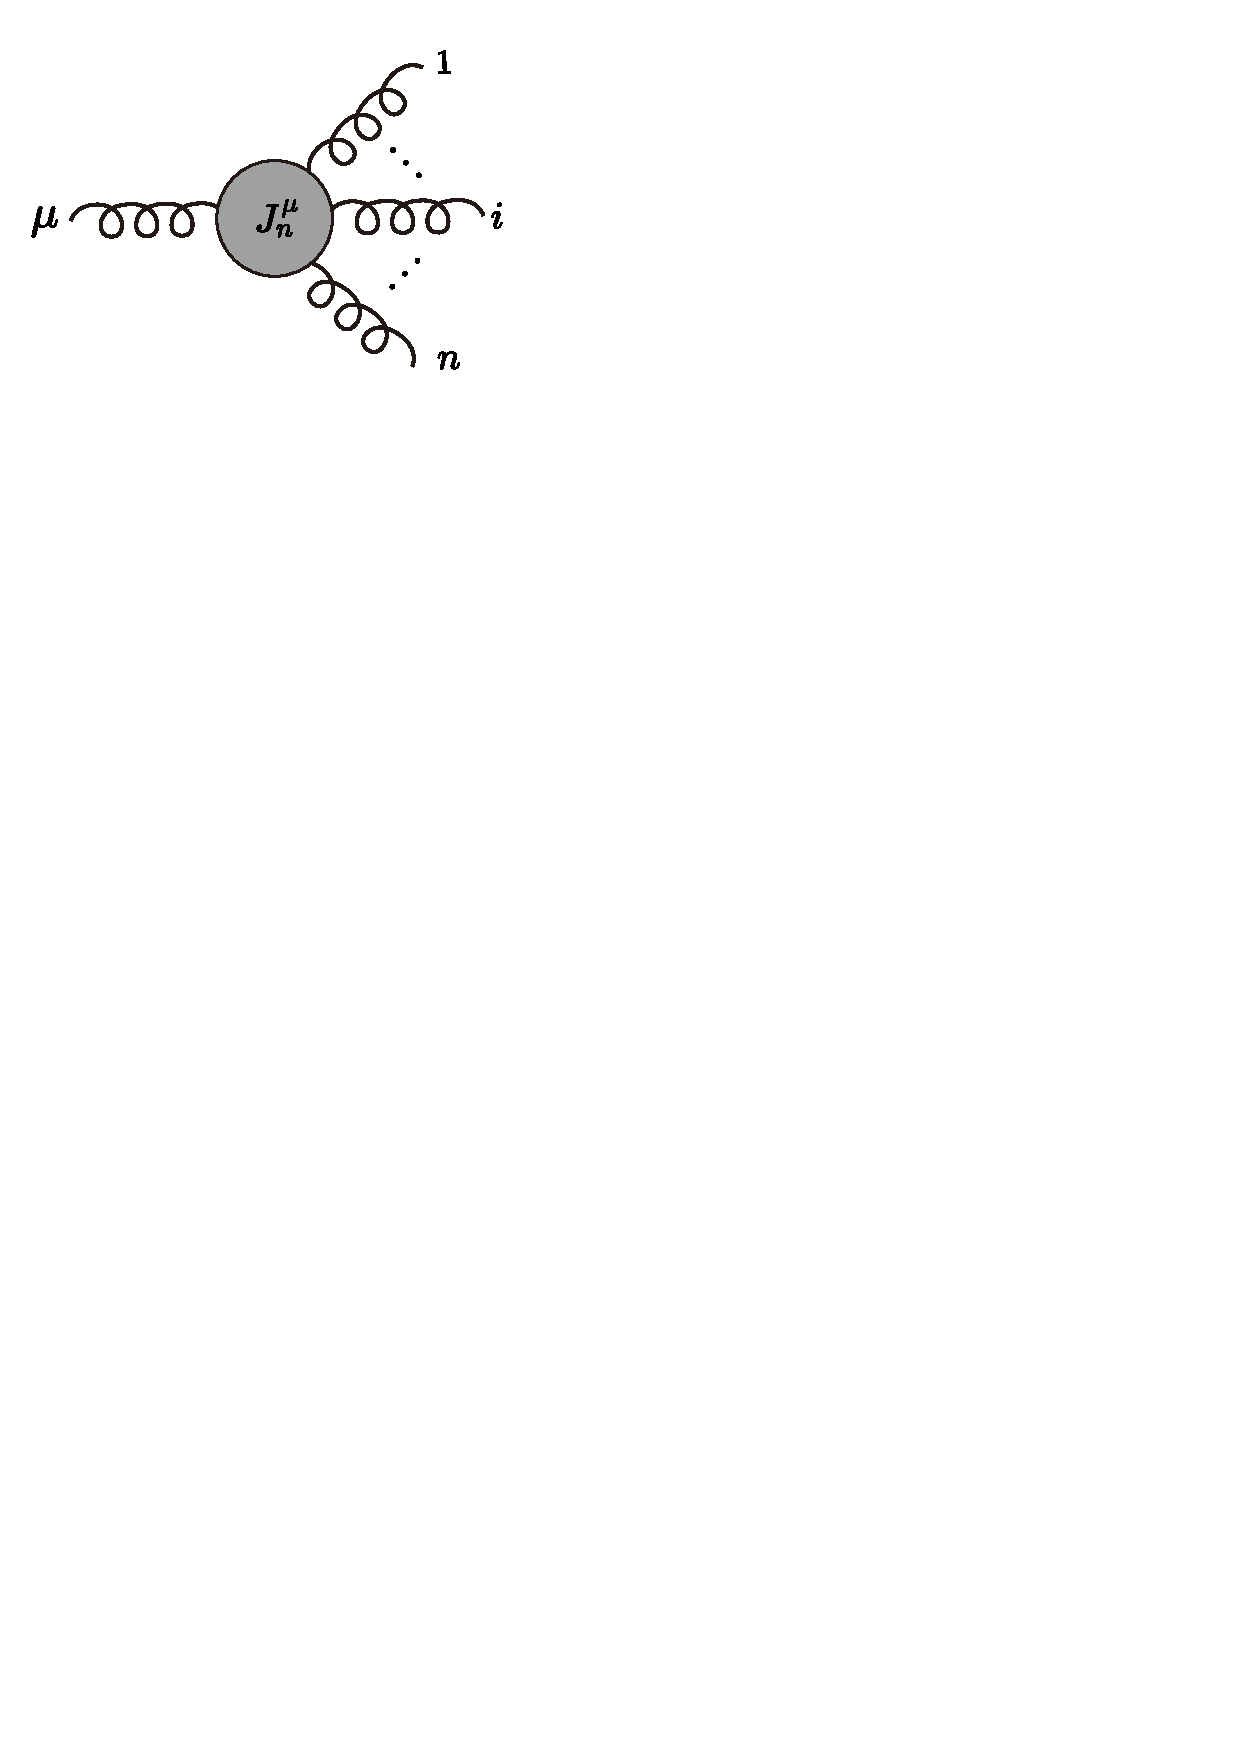
\includegraphics[width=.5\linewidth]{figs/fig13.pdf}
	\caption{BG流的定义}
	\label{fig:6.6}
\end{figure}
\begin{figure}[htbp]
	\centering
	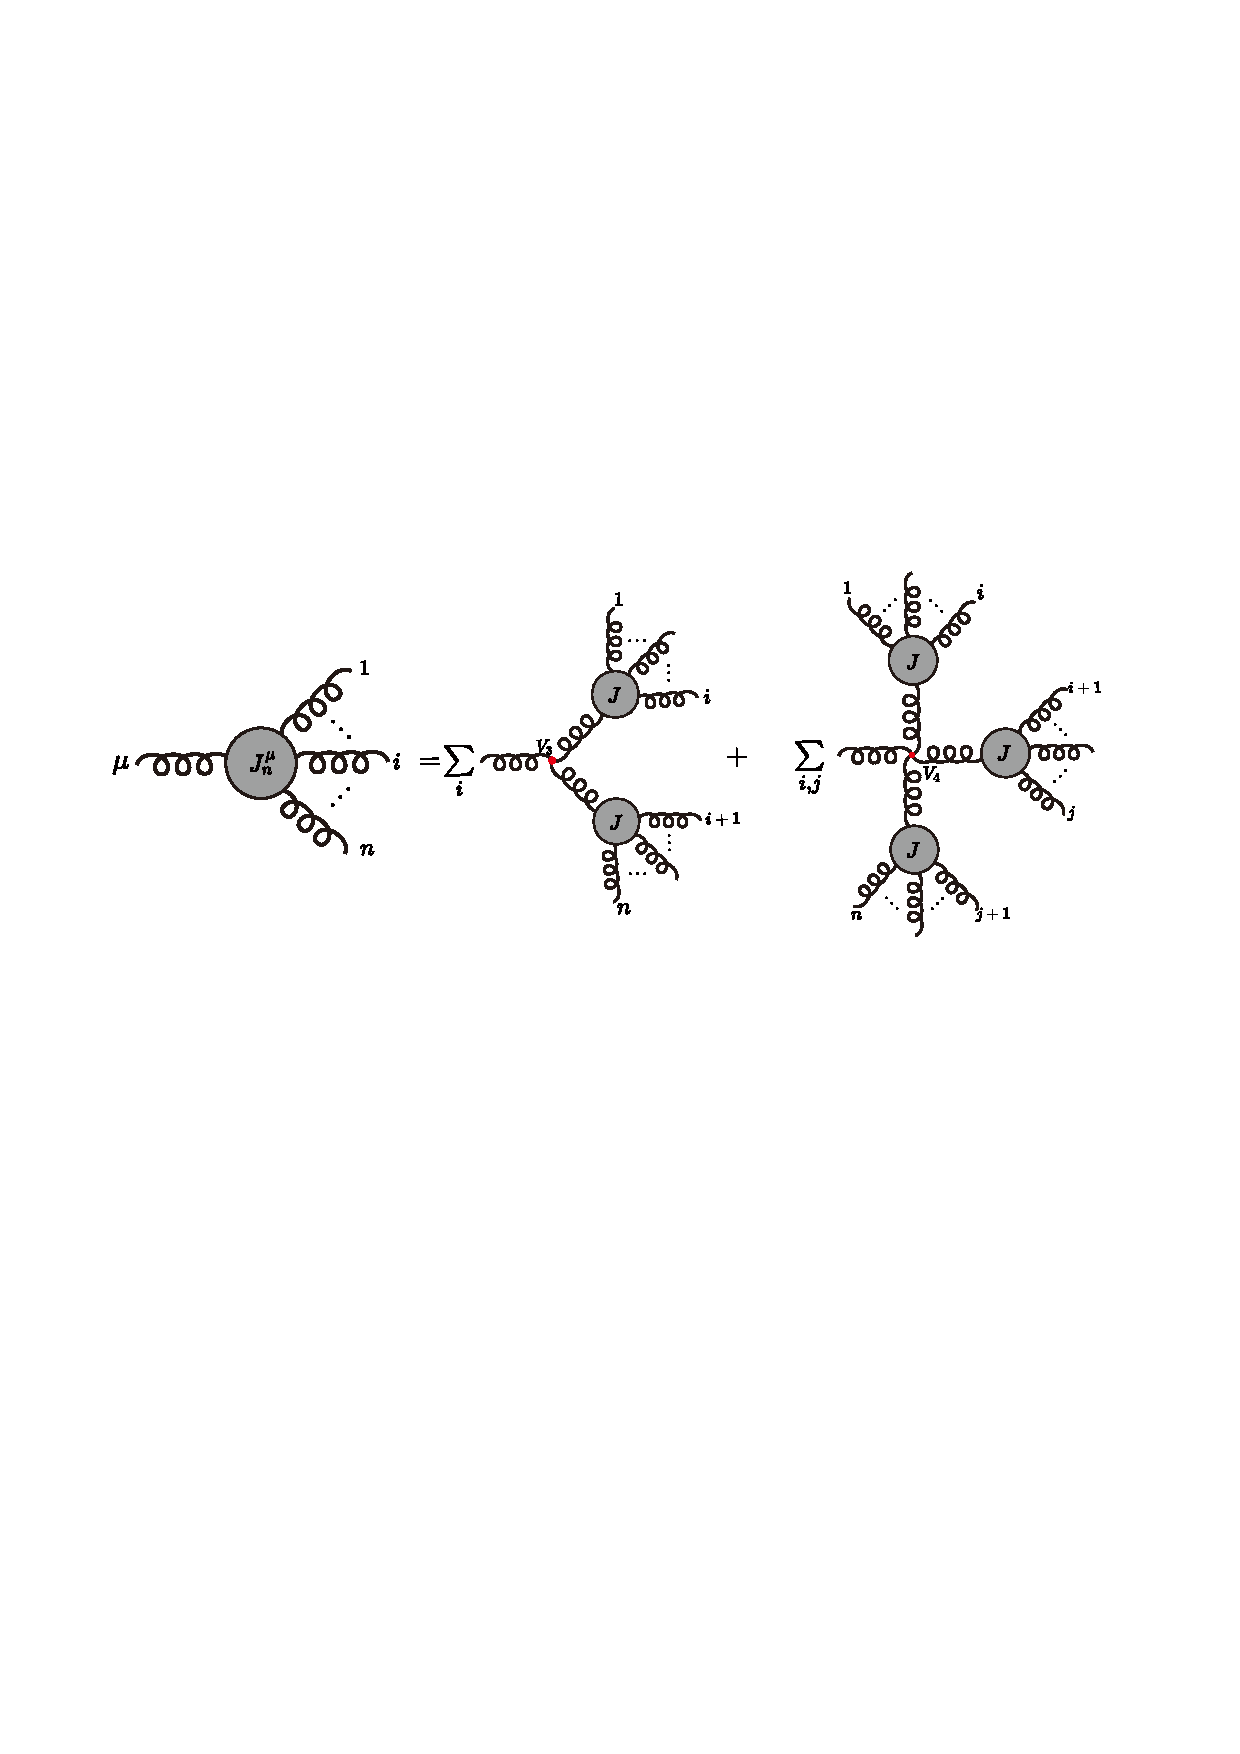
\includegraphics[width=\linewidth]{figs/fig14.pdf}
	\caption{BG流的递推关系}
	\label{fig:6.7}
\end{figure}
从BG流的定义可以直接得到:
\begin{equation}
	\mathcal{A}_{n+1} =\lim_{k^2_{n+1}=0} \epsilon^\mu_{n+1}s_{1\cdots n}J_n
\end{equation}

所以只要通过离壳递推的方式计算出BG流,就能计算出振幅本身,类似的也可以定义色序振幅BG流。显然,这种递推是极其低效的,尽管如此这种方法还是率先用于计算得到了$n$点胶子MHV振幅的Park-Taylor公式\cite{Dixon:1996wi,Mangano:1990by}。场论树级振幅本质上是在求解经典运动方程,所以BG流应当也可以从经典运动方程求解得到,这发展成了Perturbiner方法,文献\cite{Mizera:2018jbh}中有不错的介绍。

比如对于Yang-Mills理论,考虑色序振幅BG流,Yang-Mills方程为:
\begin{equation}
	\square\mathbb{A}^{\mu}=[\mathbb{A}_{\nu},\partial^{\nu}\mathbb{A}^{\mu}+\mathbb{F}^{\nu\mu}]
\end{equation}
然后取拟设:
\begin{equation}
	\mathbb{A}^\mu(x):=\sum_PA_P^\mu T^Pe^{k_P\cdot x}=\sum_iA_i^\mu T^{a_i}e^{k_i\cdot x}+\sum_{i,j}A_{ij}^\mu T^{a_i}T^{a_j}e^{k_{ij}\cdot x}+\ldots
\end{equation}
从物理上看无非就是在壳粒子取平面波拟设,$T$是在壳粒子带的色因子,而前面的$A$便是一条外腿离壳得来的平面波。所以可以通过平面波拟设解方程的方式得到BG流。

用同样的方法解(非线性)超场方程\ref{eq:5.43}可以得到SYM的BG流$\mathcal{K}_P=\frac{1}{s_P}\sum\limits_{XY=P}\mathcal{K}_{[X,Y]}$:\cite{Lee:2015upy}
\begin{equation}
	\begin{aligned}
		&\mathcal{A}_{\alpha}^{[P,Q]}=\frac{1}{2}\left[\mathcal{A}_\alpha^  {Q}(k_Q\cdot\mathcal{A}_P)+\mathcal{A}_  {Q}^m(\gamma_m\mathcal{W}_P)_\alpha-(P\leftrightarrow  {Q})\right],\\&\mathcal{A}_{[P,  {Q}]}^m=\frac{1}{2}\left[\mathcal{A}_Q^m(k_Q\cdot\mathcal{A}_P)+\mathcal{A}_n^Q\mathcal{F}_P^{mn}+(\mathcal{W}_P\gamma^m\mathcal{W}_  {Q})-(P\leftrightarrow  Q)\right],\\&\mathcal{W}_{[P,  {Q}]}^{\alpha}=\frac{1}{2}\left[\mathcal{W}_Q^\alpha(k_Q\cdot\mathcal{A}_P)+\mathcal{W}_Q^{m\alpha}\mathcal{A}_P^m+\frac{1}{2}\mathcal{F}_P^{rs}(\gamma_{rs}\mathcal{W}_Q)^\alpha-(P\leftrightarrow  Q)\right],\\&\mathcal{F}_{[  {P},  {Q}]}^{mn}=\frac{1}{2}\left[\mathcal{F}_{  {Q}}^{mn}(k_{  {Q}}\cdot\mathcal{A}_{  {P}})+\mathcal{F}_{  {Q}}^{p|mn}\mathcal{A}_{p}^{p}+\mathcal{F}_{  {Q}}^{[m}{}_{r}\mathcal{F}_{P}^{n]r}+2(\mathcal{W}_{  {Q}}\gamma^{[m}\mathcal{W}_{P}^{n]})-(P\leftrightarrow  Q)\right]
	\end{aligned}
\end{equation}
递推起点为$\mathcal{K}_i = K_i$,同样BG流由于是离壳的,所以也涉及到规范的选取,如果递推起点改为$\mathcal{K}_i = \hat{K}_i$就是在Lorenz规范下的BG流。而且可以自然退化到YM理论的BG流$\mathcal{A}_{P}^{m}(\theta=0)|_{\chi_{i}=0}=J_{P}^{m}$。利用上面的递推式计算前三个BG流得到:\footnote{注意我们只是对BCJ超场取了$\ell(P):= P$的符号约定,这里BG流的下标只是单独的一个字词。}
\begin{equation}
	\begin{aligned}
		\mathcal{ K}_{12}^{m}&=\frac{ K_{[1,2]}^m}{s_{12}}\\
		\mathcal{ K}_{123}^{m}&=\frac{ K_{[[1,2],3]}^m}{s_{12}s_{123}}+\frac{ K_{[1,[2,3]]}^m}{s_{123}s_{23}}\\
		\mathcal{ K}_{1234}^m&=\frac{ K_{[[[1,2],3],4]}^m}{s_{12}s_{123}s_{1234}}+\frac{ K_{[[1,[2,3]],4]}^m}{s_{123}s_{1234}s_{23}}+\frac{ K_{[[1,2],[3,4]]}^m}{s_{12}s_{1234}s_{34}}+\frac{ K_{[1,[[2,3],4]]}^m}{s_{1234}s_{23}s_{234}}+\frac{ K_{[1,[2,[3,4]]]}^m}{s_{1234}s_{234}s_{34}}
	\end{aligned}
\end{equation}
递归定义平面二叉树求和\cite{Mafra:2020qst},示例见图\ref{fig:6.8}:\footnote{$s_P:=\frac12 k_P^2$,注意我们本章选取了$ik\to k$的符号约定,所以后面计算结果中$s_P\to -s_P$才得到保留虚数单位时的符号约定。}
%% 在后面也要写一下
\begin{equation}
	b(P):=\frac{1}{s_P}\sum_{XY=P}[b(X),b(Y)],\quad b(i):=i,\quad b(\varnothing):=0
\end{equation}
\begin{figure}[htbp]
	\centering
	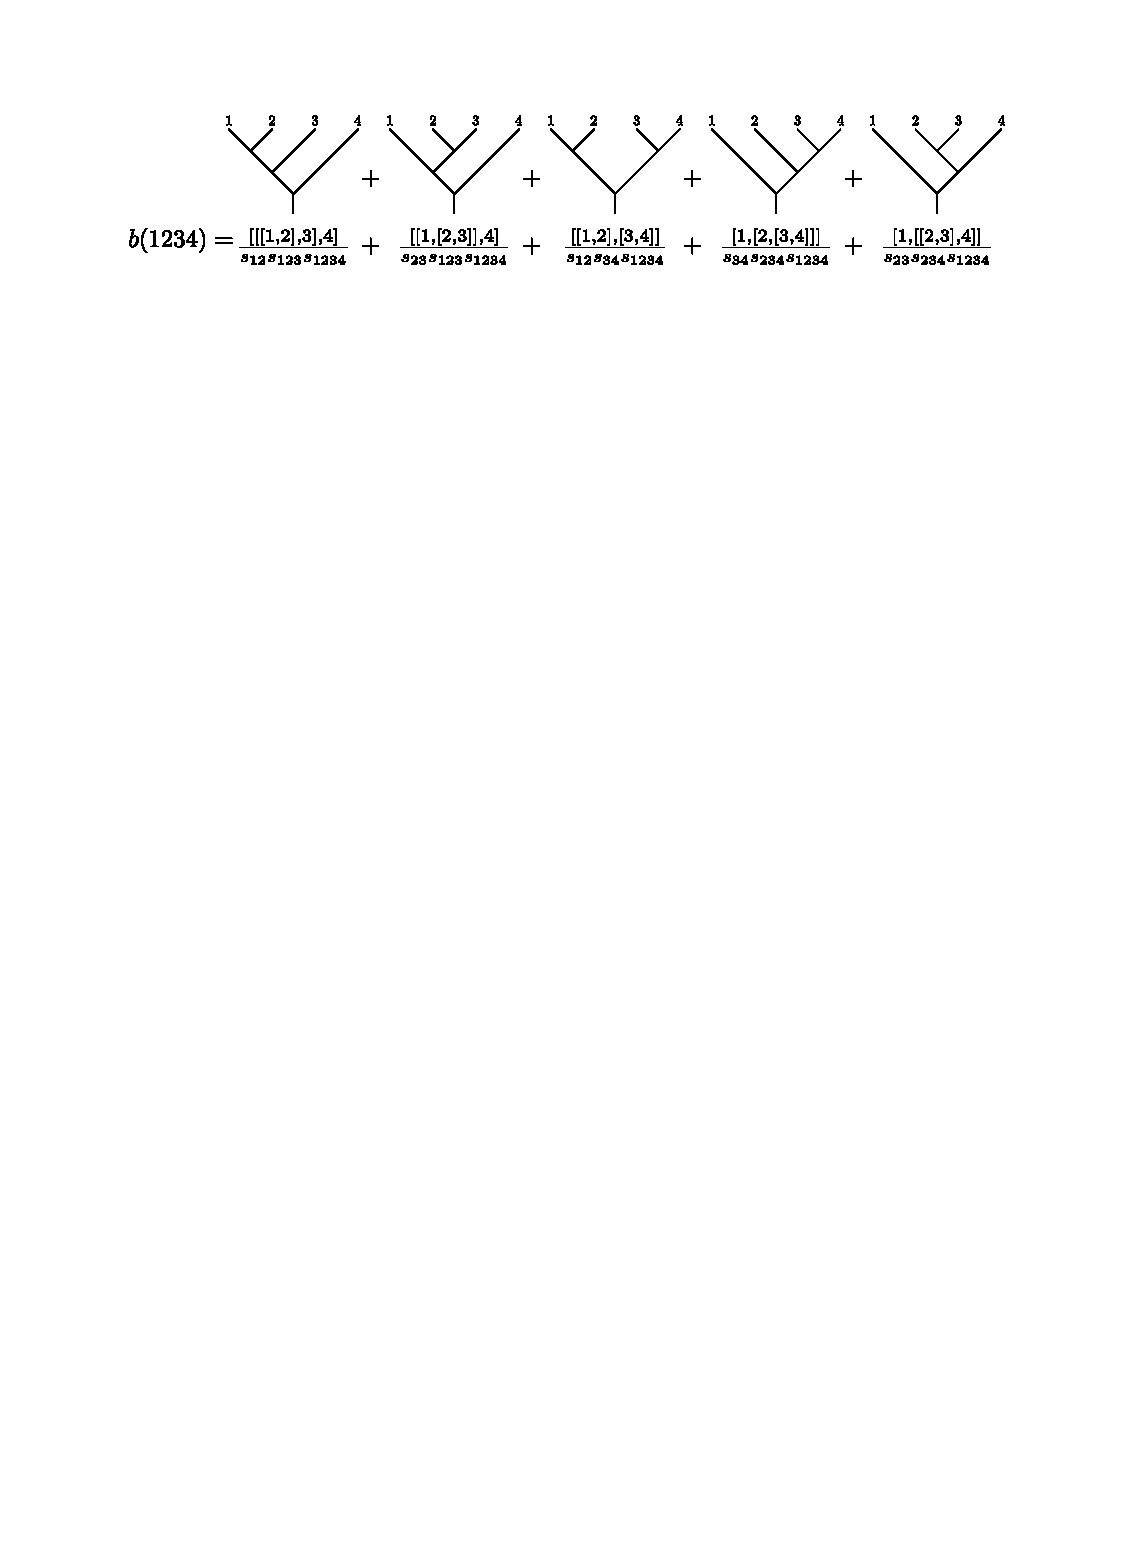
\includegraphics[width=\linewidth]{figs/fig15.pdf}
	\caption{平面二叉树求和}
	\label{fig:6.8}
\end{figure}
所以BG流和超场之间可以用下面的等式联系:
\begin{equation}
	\boxed{
		\mathcal{K}_P=K_{b(P)}
	}
\end{equation}
同理对Lorenz规范有$\mathcal{K}_P=K_{b(P)}$,这不仅能简化计算,后面会看到BG流的对称性可以从$b$算符本身的对称性很快得出。

但是后面构造SYM振幅并不用超场对应的这个BG流$\mathcal{K}$构造,而是利用纯旋量空间的类似物:
\begin{equation}
	M_P=\lambda^\alpha\mathcal{A}_\alpha^P
\end{equation}
这个是后面递推会用到的BG流。同理有$M_P=V_{b(P)}$。
\subsection{自由李代数对称性}
平面二叉树映射有个很重要的性质是自伴性:
\begin{equation}
	\label{eq:6.55}
	\langle b(P),Q\rangle=\langle P,b(Q)\rangle
\end{equation}
其证明只要注意到:
\begin{equation}
\begin{gathered}
		\langle b(P),Q\rangle=\frac{1}{s_P}\sum_{XY=P}\langle b(X)b(Y),Q\rangle-(X\leftrightarrow Y)\\
	\langle AB,RS\rangle=\langle A,R\rangle\langle B,S\rangle,\quad|A|=|R|,\quad|B|=|S|
\end{gathered}
\end{equation}
然后对$|P|$进行数学归纳便可得证,洗牌序有下面的重要定理:
\begin{boxedtext}[Ree定理]
	任取非空字词$\Gamma$,$R$和$S$,满足下式:
	\begin{equation}
		\langle\Gamma,R\shuffle S\rangle=0,\quad R,S\neq\varnothing
	\end{equation}
\end{boxedtext}
利用\ref{eq:6.55}以及Ree定理立刻得到:
\begin{equation}
\begin{aligned}
	\label{eq:6.58}
		&0=\langle b(P),R\shuffle S\rangle=\langle P,b(R\shuffle S)\rangle,\quad R,S\neq\emptyset,\quad\forall P\\
	\Rightarrow &b(A\shuffle B)=0,\quad\forall A,B\neq\emptyset
\end{aligned}
\end{equation}
这意味着BG流有下面的对称性:
\begin{equation}
	\mathcal{K}_{A\shuffle B}=0,\quad\forall A,B\neq\varnothing
\end{equation}
这是BG流非常重要的对称性,从这里看来只是自由李代数的简单应用,文献\cite{Frost:2020eoa}中有更多类似的讨论,其中$S$括号$\{\bullet,\bullet\}$的定义比较有用:
\begin{equation}
	\{P,Q\}=\sum_{\substack{XiY=P\\{ { {RjS=Q}}}}}k_i\cdot k_j(X \shuffle\tilde{Y})ij(\tilde{R} \shuffle S)(-1)^{|Y|+|R|}
\end{equation}
注意$S$括号定义在$\mathcal{L}^*\times \mathcal{L}^*\to\mathcal{L}^*$,$\mathcal{L}$是李多项式所在的线性空间$\mathcal{L}^*$是其对偶空间,在这里我们可以理解为商空间$\mathcal{L}/\sim$,其中:
\begin{equation}
	A\sim B\Leftrightarrow A=B+\sum R\shuffle  S,R,S\neq\varnothing
\end{equation}
$S$括号有下面的性质:
\begin{equation}
	\label{eq:6.62}
	\{A\shuffle B,C\}=0,\quad b(\{P,Q\})=[b(P),b(Q)],\quad \sum_{XY=P}\{X,Y\}\sim s_PP
\end{equation}
而且$S$括号实际上是$C$映射的伴随算子:
\begin{equation}
	\langle P\otimes Q,C(\Gamma)\rangle=\langle\{P,Q\},\Gamma\rangle
\end{equation}
$C$映射有下面重要的恒等式:
\begin{align}
	C(\ell(P))&=\sum_{\substack{XjY=P\\\delta(Y)=R\otimes S}}(k_X\cdot k_j)\left[\ell(XR)\otimes\ell(jS)-\ell(jR)\otimes\ell(XS)\right]\notag\\
	&=\sum_{\substack{XjY=P\\\delta(Y)=R\otimes S}}(k_X\cdot k_j)\ell(XR)\wedge\ell(jS)\\
	C(P\wedge Q)&=C(P)\wedge Q-P\wedge C(Q)\\
	\label{eq:6.66}
	C\left(b(P)\right)&=\sum_{XY=P}\left(b(X)\otimes b(Y)-b(Y)\otimes b(X)\right):=\sum_{XY=P}b(X)\wedge b(Y)
\end{align}
利用第上面第一个等式:
\begin{equation}
	C(\ell(123))=(k_1\cdot k_2)\left(\ell(1)\wedge\ell(23)+\ell(13)\wedge\ell(2)\right)+(k_{12}\cdot k_3)\ell(12)\wedge\ell(3)
\end{equation}
再利用\ref{eq:6.46},并且注意到$V_P:=V_{\ell(P)}$:
\begin{equation}
	QV_{123}=(k_1\cdot k_2)\left(V_1V_{23}+V_{13}V_2\right)+(k_{12}\cdot k_3)V_{12}V_3
\end{equation}
可以看到两式数学结构完全一致!$VV$之间的OPE乘法在自由李代数中被替换为了反对易的$\wedge$,而$V$恰好是费米算符!而且从组合学上可以证明$C^2=0$。结合前面所有的讨论,我们可以断言超场之于下标的作用正如$C$,$\ell$和$b$之于字词的作用:
\begin{equation}
	\label{eq:6.69}
	\boxed{
		C\leftrightarrow Q_{\mathrm{BRST}},\quad\ell(P)\leftrightarrow V_P/K_P,\quad b(P)\leftrightarrow M_P/\mathcal{K}_P
	}
\end{equation}
这就是BG流/多粒子超场和自由李代数之间的深刻关联。对于$\ell(P)$形式的多粒子顶角算符,\ref{eq:6.46}其实可以改写为:
\begin{equation}
	QV_\Gamma:=QV_\ell(\Gamma)=(V\wedge V)_{\mathbb{C}(\Gamma)}
\end{equation}
现在利用\ref{eq:6.66}得到:
\begin{equation}
	\label{eq:6.71}
\begin{aligned}
		QM_P&=QV_{b(P)}=(V\wedge V)_{C(b(P))}=\sum_{XY=P}(V\wedge V)_{b(X)\wedge b(Y)}=\sum_{XY=P}V_{b(X)}V_{b(Y)}\\
	&=\sum_{XY=P}M_XM_Y
\end{aligned}
\end{equation}
还有一个比较重要的KLT映射,我们用$\mathcal{S}:\mathcal{L}\to\mathcal{L}^*$表示,他的定义是将所有$\Gamma$中的李括号$[\bullet,\bullet]$改为$S$括号$\{\bullet,\bullet\}$,变换后的李多项式记作$\{\Gamma\}$。由此定义广义KLT核:
\begin{equation}
	\mathcal{S}^\ell(P| Q)=\langle\{\ell(P)\},\ell( Q)\rangle
\end{equation}
KLT关系中的固定$i,n-1,n$三条外腿的KLT核是上面的特殊形式:
\begin{equation}
	S(P|Q)_i=S^\ell(iP|iQ)
\end{equation}
其满足下面的递推式:\cite{Carrasco:2016ldy}
\begin{equation}
	S(Aj|BjC)_i=k_j\cdot k_{iB}S(A|BC)_i,\quad S(\varnothing|\varnothing)_i:=1
\end{equation}
KLT映射和$b$映射之间互逆,也就是说
\begin{equation}
	\label{eq:6.75}
	\mathcal{S}\circ b = \mathrm{id}_{\mathcal{L}^*},\quad b\circ \mathcal{S} = \mathrm{id}_{\mathcal{L}}
\end{equation}
一个词$P$称为是Lyndon的当且仅当在所有的$\mathrm{cyc}(P)$中$P$在字典序的意义下最小。Lyndon词可以作为$\mathcal{L}^*$的一组基底,$\ell(P)$则是$\mathcal{L}$的一组自然基底。所以$\{\ell(P)\}$可以在Lyndon基底下展开:\footnote{严格来说因为$\mathcal{L}^*$是在商空间的意义下定义的,下面的$=$应当替换为$\sim$。}
\begin{equation}
	\label{eq:6.76}
	\{\ell( {P})\}=\sum_{ {Q}\in \mathrm{Lyndon}}\langle\{\ell( {P})\},\ell( {Q})\rangle {Q}
\end{equation}
等式两边作用$b$映射并利用\ref{eq:6.75}得到:
\begin{equation}
	\ell(P)=b(\{\ell(  {P})\})=\sum_{  {Q}\in\mathrm{Lyndon}}\langle\{\ell(  {P})\},\ell(  {Q})\rangle b(  {Q})=\sum_QS^\ell(P|iQ)b(iQ)
\end{equation}
这里最后一个等号利用KLT核只有在$P$和$Q$中元素相同时不为零简化了求和计算,$i$是$P$中最小的字,$Q$表示$P/\{i\}$的字组成的词。把$P$也改写为$iP$ Lyndon词的形式,并利用\ref{eq:6.69}给出的对应得到:
\begin{equation}
	\label{eq:6.78}
	V_{iP}=\sum_{Q}S(P|Q)_iM_{iQ},\quad K_{iP}=\sum_{Q}S(P|Q)_i\mathcal{K}_{iQ}
\end{equation}
同样利用\ref{eq:6.76}类似的基底展开式可以证明下面的Schocker恒等式:
\begin{equation}
	\label{eq:schocker}
	B i A \sim (-1)^{|B|} i (A \shuffle\tilde{B})
\end{equation}
再利用\ref{eq:6.69}的对应,只有$b$才能除去等价模掉的$R\shuffle S$的影响(\ref{eq:6.58}),给出:
\begin{equation}
	\label{schocker}
	\mathcal{K}_{B1A}=(-1)^{|B|}\mathcal{K}_{1(A\shuffle\tilde{B})}
\end{equation}
对$M$也同样成立。

回到一开始为了简化OPE的想法,我们研究了这么多多粒子超场的性质,都是为了顶角算符OPE变得有规律些:
\begin{equation}
	\label{eq:6.79}
	V_A(z_a)U_B(z_b)\to\frac{V_{[A,B]}(z_b)}{z_{ab}},\quad U_A(z_a)U_B(z_b)\to\frac{U_{[A,B]}(z_b)}{z_{ab}}
\end{equation}
这种简化后的OPE使得超弦$n$点盘面振幅计算变得可能。

\section{超弦无质量态$n$点盘面振幅}
取$z_n=\infty$的约定,现在利用\ref{eq:6.79}进行类似$\S$\ref{sec:5.4}的计算,只是顶角算符被看作了一个整体,比如四点OPE:
\begin{equation}
	\label{eq:6.80}
	\begin{aligned}
		V_1(z_1)U_2(z_2)V_3(z_3)V_4(\infty)&=\wick{\c V_1\c U_2V_3V_4}+\wick{ V_1\c U_2\c V_3V_4}+\wick{V_1\c U_2V_3\c V_4}\\
		&\cong\frac{V_{[1,2]}(z_1)}{z_{12}}V_3(z_3)V_4(\infty)+V_1(z_1)\frac{V_{[2,3]}(z_3)}{z_{23}}V_4(\infty)\\&\cong\frac{V_{12}V_3V_4}{z_{12}}+\frac{V_1V_{32}V_4}{z_{32}}
	\end{aligned}
\end{equation}
第二步利用了$z_4\to\infty$,所以任何与$V_4$的OPE均会被压低,第三步利用了$VV$之间OPE平凡。类似的对$n$点情况计算得到OPE:
\begin{equation}
	V_1\cdots U_i\cdots V_{n-1}V_n\cong\sum_{AB=23...n-2}(V_{1A}\mathcal{Z}_{1A})(V_{n-1,\tilde{B}}\mathcal{Z}_{n-1,\tilde{B}})V_n+\mathrm{perm}(2,3,...,n-2)
\end{equation}
其中$\mathcal{Z}$因子定义为:
\begin{equation}
	\label{PT}
	\mathcal{Z}_{123...p}:=\frac{1}{z_{12}z_{23}\ldots z_{p-1,p}}=z_{p1}\cdot\mathrm{PT}(1,2,\cdots,p)
\end{equation}
类似在RNS超弦振幅计算中所做的,对关联函数取不同盘面顺序积分得到相应的色序振幅,只不过我们这里还需要额外对零模积分:
\begin{equation}
	\label{eq:6.85}
\boxed{
		\mathcal{A}_n(P)=(2\alpha^{\prime})^{n-3}\int d\mu_P^n\sum_{AB=23...n-2}\langle\left(V_{1A}\mathcal{Z}_{1A}\right)(V_{(n-1)\tilde{B}}\mathcal{Z}_{n-1,\tilde{B}})V_n\rangle+\mathrm{perm}(23\ldots n-2)
}
\end{equation}
这里积分测度为带Koba-Nielsen因子的$SL(2,\mathbb{R})$不变测度:\footnote{似乎和前面$\S$4计算出来的KN因子不同,这是因为我们选取了$ik\to k$的符号约定,所以$s\to -s$。}
\begin{equation}
	\int d\mu_P^n:=\int_{D(P)}dz_2dz_3\cdots dz_{n-2}\prod_{1\leq i<j}^{n-1}|z_{ij}|^{-2\alpha^{\prime}s_{ij}}
\end{equation}
同样$z_1$和$z_{n-1}$的坐标约定选取$\{0,1\}$或$\{1,0\}$应当与排序$P$相容。比如利用\ref{eq:6.80},四点振幅为:
\begin{equation}
	\begin{aligned}
		\mathcal{A}(1,2,3,4)&=2\alpha^{\prime}\int_0^1dz_2\left(\frac{\langle V_{12}V_3V_4\rangle}{z_{12}}+\frac{\langle V_1V_{32}V_4\rangle}{z_{32}}\right)|z_{12}|^{-2\alpha^{\prime}s_{12}}|z_{23}|^{-2\alpha^{\prime}s_{23}}\\&=\left(\frac{\langle V_{12}V_3V_4\rangle}{s_{12}}+\frac{\langle V_1V_{23}V_4\rangle}{s_{23}}\right)\frac{\Gamma(1-2\alpha^{\prime}s_{12})\Gamma(1-2\alpha^{\prime}s_{23})}{\Gamma(1-2\alpha^{\prime}s_{12}-2\alpha^{\prime}s_{23})}
	\end{aligned}
\end{equation}
定义一个同样对下标满足广义BCJ恒等式\ref{eq:6.38}的变量:
\begin{equation}
	X_{P}:=\frac{1}{|P|}\sum_{ {Q}}S^{\ell}(P| {Q})\mathcal{Z}_{ {Q}}=\prod_{j=2}^{|P|}\sum_{i=1}^{j-1}\frac{s_{p_ip_j}}{z_{p_ip_j}}
\end{equation}
其满足下面的积分恒等式:
\begin{equation}
	\label{eq:6.87}
	\int d\mu_P^nX_{1A}X_{(n-1)\tilde{B}}=(-1)^{|B|}\int d\mu_P^nX_{1AB}
\end{equation}
我们举五点的例子来说明,首先注意到由于KN因子包含每两个点坐标之差,所以有:
\begin{equation}
	\int_{z_a}^{z_b}dz_k\frac{\partial}{\partial z_k}\frac{\prod_{1\leq i<j}^{n-1}|z_{ij}|^{-2\alpha^{\prime}s_{ij}}}{z_{i_1j_1}\cdots z_{i_{n-4}j_{n-4}}}=0
\end{equation}
考虑$z_k$不在分母中出现的特殊情况,比如五点情况作用$\partial_{z_3}$得到:
\begin{equation}
	\int_{D(P)}dz_2dz_3\prod_{1\leq i<j}^4|z_{ij}|^{-2\alpha^{\prime}s_{ij}}
	\eqnmarkbox[blue]{node1}{\frac{s_{12}}{z_{12}}\left(\frac{s_{13}}{z_{13}}+\frac{s_{23}}{z_{23}}\right)}
	=\int_{D(P)}dz_2dz_3\prod_{1\leq i<j}^4|z_{ij}|^{-2\alpha^{\prime}s_{ij}}
	\eqnmarkbox[red]{node2}{\frac{s_{12}}{z_{12}}\frac{s_{34}}{z_{34}}}
\end{equation}
\annotate[yshift=0em]{below,left}{node1}{$X_{123}$}
\annotate[yshift=+0.5em]{above,left}{node2}{$X_{12}\cdot X_{34}$}
将\ref{eq:6.87}与\ref{schocker}结合得到:
\begin{equation}
	\int d\mu_P^n(M_{1A}X_{1A})(M_{n-1\tilde{B}}X_{(n-1)\tilde{B}})=\int d\mu_P^nX_{1AB}M_{1A}M_{B(n-1)}
\end{equation}
另外从\ref{eq:6.78}可以看到:
\begin{equation}
	\sum_AV_{iA}Z_{iA}=\sum_AM_{iA}X_{iA}
\end{equation}
利用这两个式子就能将\ref{eq:6.85}改用$M_P$表达,比如四点情况:
\begin{equation}
\begin{aligned}
		\mathcal{A}_4(P)&=2\alpha^{\prime}\int d\mu_P^4\left\langle V_{12}\mathcal{Z}_{12}V_3V_4+V_1V_{32}\mathcal{Z}_{32}V_4\right\rangle\\
	&=2\alpha^{\prime}\int d\mu_{P}^{4}\left\langle X_{12}M_{12}M_{3}M_{4}+X_{32}M_{1}M_{32}M_{4}\right\rangle\\
	&=2\alpha^{\prime}\int d\mu_P^4X_{12}\langle M_{12}M_3M_4+M_1M_{23}M_4\rangle
\end{aligned}
\end{equation}
对于任意点有:
\begin{equation}
\boxed{
		\mathcal{A}_n(P)=(2\alpha^{\prime})^{n-3}\int d\mu_P^n\left[\prod_{k=2}^{n-2}\sum_{m=1}^{k-1}\frac{s_{mk}}{z_{mk}}A_n(1,2,\ldots,n)+\mathrm{perm}(2,3,\ldots,n-2)\right]
}
\end{equation}
其中:
\begin{equation}
	\label{eq:6.96}
\boxed{
		A_n(P,n):=\sum_{XY=P}\langle M_XM_YM_n\rangle
}
\end{equation}
考虑固定三个外腿顺序的情况:
\begin{equation}
	\mathcal{A}_n(1,R,n-1,n;\alpha^{\prime})=\sum_{{Q}\in S_{n-3}}{{F}_R}^{Q}(\alpha^{\prime})A_n(1,{Q},n-1,n)
\end{equation}
其中:
\begin{equation}
\begin{aligned}
	\label{eq:6.98}
		{F_R}^Q(\alpha^{\prime}):=&(2\alpha^{\prime})^{n-3}\int d\mu_R^n\frac{s_{1q_2}}{z_{1q_2}}\left(\frac{s_{1q_3}}{z_{1q_3}}+\frac{s_{q_2q_3}}{z_{q_2q_3}}\right)
	\times\left(\frac{s_{1q_4}}{z_{1q_4}}+\frac{s_{q_2q_4}}{z_{q_2q_4}}+\frac{s_{q_3q_4}}{z_{q_3q_4}}\right)\cdots\\
	&\times\left(\frac{s_{1q_{n-2}}}{z_{1q_{n-2}}}+\frac{s_{q_2q_{n-2}}}{z_{q_2q_{n-2}}}+\cdots+\frac{s_{q_{n-3}q_{n-2}}}{z_{q_{n-3}q_{n-2}}}\right)
\end{aligned}
\end{equation}
\section{SYM振幅的纯旋量超空间上同调表述}
利用下面$\alpha'\to 0$的展开式:
\begin{equation}
	\log\Gamma(1-z)=\gamma z+\sum_{n=2}^\infty\frac{z^n}{n}\zeta_n
\end{equation}
$\gamma$是Euler常数,$\zeta$是黎曼$\zeta$函数,对四点情况展开\ref{eq:6.98}:
\begin{equation}
\begin{aligned}
		{F_2}^2&=\frac{\Gamma(1-2\alpha^{\prime}s_{12})\Gamma(1-2\alpha^{\prime}s_{23})}{\Gamma(1-2\alpha^{\prime}s_{12}-2\alpha^{\prime}s_{23})}=\exp\left(\sum_{n=2}^\infty\frac{\zeta_n}{n}(2\alpha^{\prime})^n\left[s_{12}^n+s_{23}^n-(s_{12}+s_{23})^n\right]\right)\\
	&=1-(2\alpha^{\prime})^2\zeta_2s_{12}s_{23}+\cdots
\end{aligned}
\end{equation}
其实,对于一般情况有:
\begin{equation}
	{F_P}^{Q}(\alpha^{\prime})=\delta_P^{Q}+\mathcal{O}({\alpha'}^2)
\end{equation}
这就说明\ref{eq:6.96}就是弦振幅的低能展开,也就是固定一个外腿$n$的SYM色序振幅!前面我们将$M_P$解释为纯旋量空间BG流的类似物,所以这里对SYM振幅的构造完全可以解释为用BG流拼凑得来,如图\ref{fig:6.9}。
\begin{figure}[htbp]
	\centering
	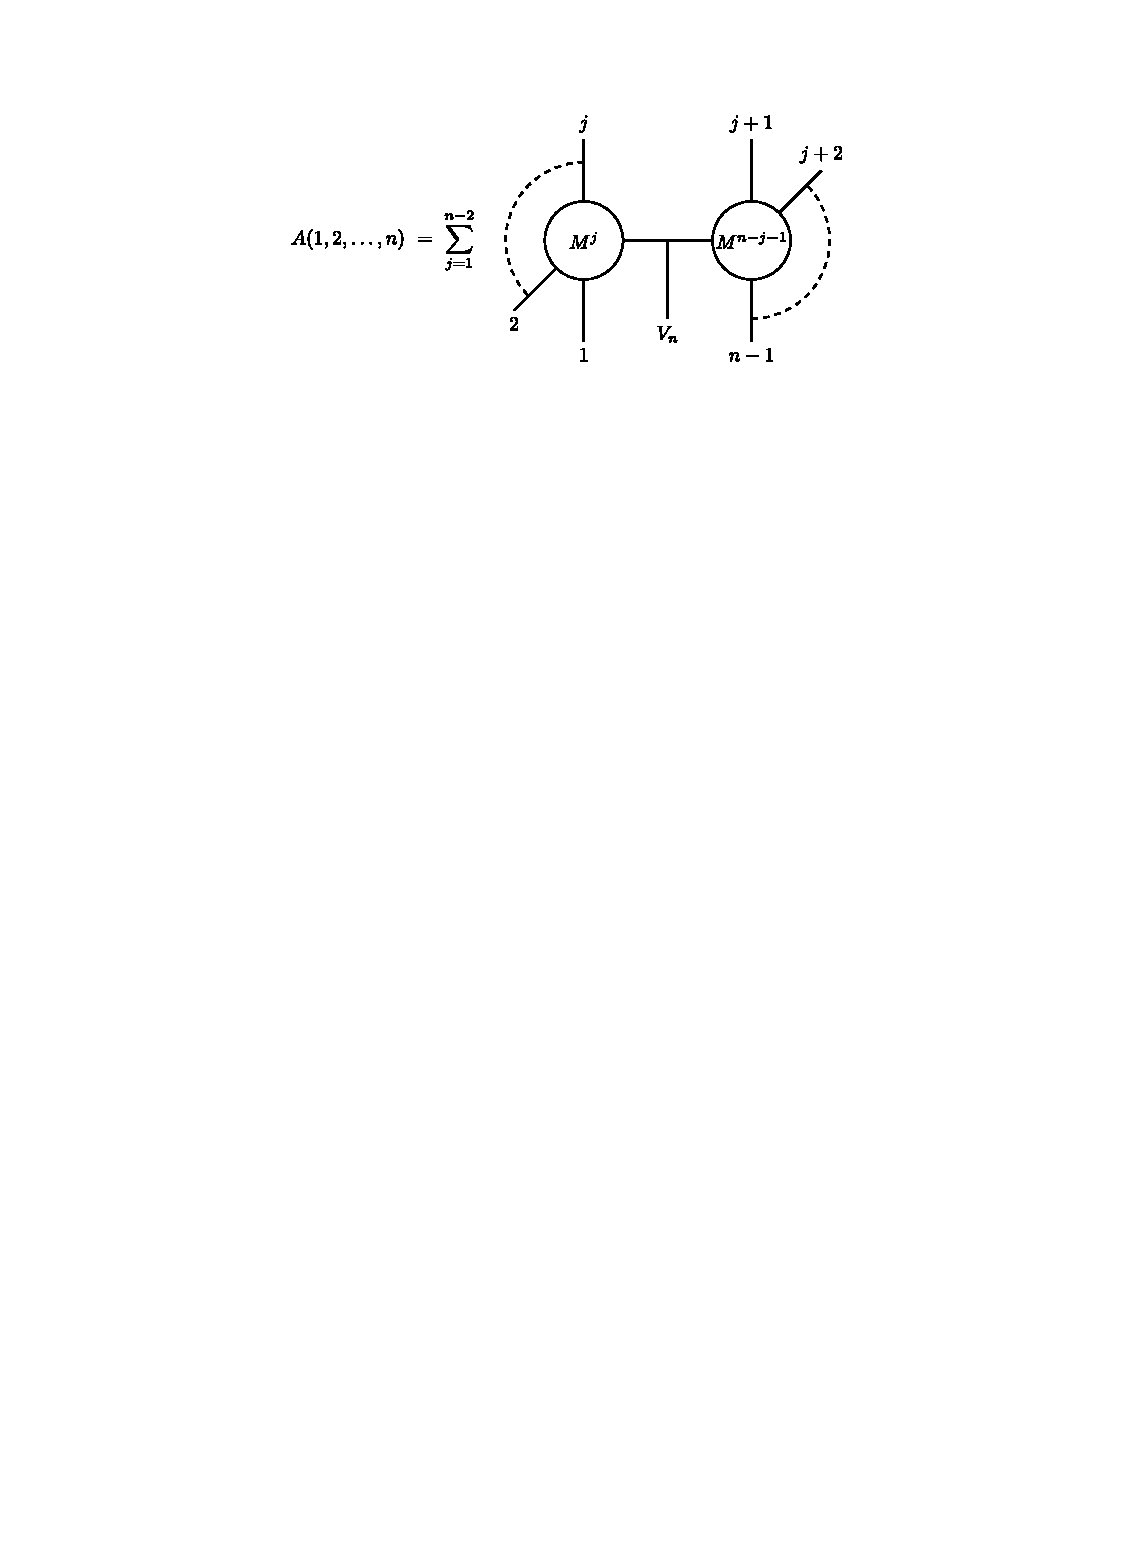
\includegraphics[width=0.8\linewidth]{figs/fig16.pdf}
	\caption{SYM振幅的纯旋量超空间上同调形式}
	\label{fig:6.9}
\end{figure}
注意到$QM_n=QV_n=0$,以及:
\begin{equation}
	\begin{aligned}
		\sum_{XY=P}Q(M_XM_Y)&=\sum_{XY=P}\sum_{RS=X}M_RM_SM_Y-\sum_{XY=P}\sum_{RS=Y}M_XM_RM_S\\&=\sum_{RSY=P}\left(M_RM_SM_Y-M_RM_SM_Y\right)=0
	\end{aligned}
\end{equation}
所以\ref{eq:6.96}是闭的,虽然看似根据\ref{eq:6.71}$E_P:=\sum_{XY=P}M_XM_Y$是恰当的,但是由于$M_P$本身的定义包含$s_P$因子,所以对于这里$s_P=k_n^2=0$,也就是在壳时\ref{eq:6.71}不是良定义的,所以在壳时无法将$\sum_{XY=P}M_XM_Y$看作是恰当的,但离壳时可以。所以用\ref{eq:6.96}形式写下的算符明显地存在于纯旋量超空间的上同调群中。但是这种表述并没有明显地满足循环对称的要求,现在我们来证明循环变换指标只会导致一个BRST恰当项的差别,在关联函数的意义下为$0$。



任意点振幅都可以通过加上一些BRST恰当的项写成循环对称的形式,比如:
\begin{equation}
	A_7(1,2,\ldots,7)=\langle M_{123}M_{45}M_{67}\rangle+\langle M_1M_{234}M_{567}\rangle+\mathrm{cyc}(12\ldots7)
\end{equation}

原则上,$M_P$可以用$\mathcal{K}_P$表达,而$\mathcal{K}_P$又可以用$K_P$表达,而多粒子超场又可以用单粒子超场表达,单粒子超场$\theta$展开是已知的,所以原则上总可以通过这种方式计算出任意点SYM振幅。上述过程其实可以进一步简化,$\mathcal{K}$的$\theta$展开是可以直接计算的,由于最终只涉及到$M_P$,所以只需要$\mathcal{A}^P_\alpha$的展开:
\begin{equation}
	\mathcal{A}_\alpha^P(\theta)=\frac{1}{2}(\theta\gamma_m)_\alpha\mathfrak{e}_P^m+\frac{1}{3}(\theta\gamma^m)_\alpha(\theta\gamma_m\mathfrak{X}_P)-\frac{1}{32}(\theta\gamma^p)_\alpha(\theta\gamma_{mnp}\theta)\mathfrak{f}_P^{mn}+\cdots
\end{equation}
其中哥特体标注的多粒子极化矢量(波函数)有递推公式:\footnote{形式上很像是“BG流的BG流”。}
\begin{align*}
	&\mathfrak{e}_P^m=\frac{1}{s_P}\sum_{XY=P}\mathfrak{e}_{[X,Y]}^m,\quad\mathfrak{X}_P^\alpha=\frac{1}{s_P}\sum_{XY=P}\mathfrak{X}_{[X,Y]}^\alpha\\
	&\mathfrak{f}_P^{mn}:=k_P^m\mathfrak{e}_P^n-k_P^n\mathfrak{e}_P^m-\sum_{XY=P}\left(\mathfrak{e}_X^m\mathfrak{e}_Y^n-\mathfrak{e}_X^n\mathfrak{e}_Y^m\right)\\
	&\mathfrak{e}_{[X,Y]}^m:=\frac{1}{2}\left[\mathfrak{e}_Y^m(k_Y\cdot\mathfrak{e}_X)+\mathfrak{e}_n^X\mathfrak{f}_Y^{nm}+( X_X\gamma^m X_Y)-(X\leftrightarrow Y)\right]\\
	& \mathfrak{X}_{[X,Y]}^\alpha:=\frac{1}{2}(k_X^p+k_Y^p)\gamma_p^{\alpha\beta}\left[\mathfrak{e}_X^m(\gamma_m \mathfrak{X}_Y)_\beta-\mathfrak{e}_Y^m(\gamma_m \mathfrak{X}_X)_\beta\right]
\end{align*}
递推起点为$\mathfrak{e}_i^m:=e_i^m$,$\mathfrak{X}_i^\alpha:=\chi_i^\alpha$。再利用附录\ref{appendix:B}给出的零模积分公式可以得到:
\begin{equation}
	\label{eq:6.105}
	\langle M_XM_YM_Z\rangle=\frac{1}{2}\mathfrak{e}_X^m\mathfrak{f}_Y^{mn}\mathfrak{e}_Z^n+(\mathfrak{X}_X\gamma_m\mathfrak{X}_Y)e_Z^m+\mathrm{cyc}(XYZ)
\end{equation}
从数值运算的角度,依赖于BG流离壳递推的这个公式要快不少。\cite{Badger:2012uz}

由于我们将振幅表述为了多粒子顶角算符,而这又根据\ref{eq:6.69}可以和自由李代数的结构联系起来,所以振幅所满足的性质应当完全可以从组合学的意义上看出。

首先是KK关系,尽管就振幅而言,由于$s_P=0$,$E_P\neq QM_P$,但是单纯从组合学上说$E_P$应当和$M_P$一样满足相同的自由李代数恒等式。比如$E_{R\shuffle S} = 0$,根据\ref{schocker}同样对$E$得到:
\begin{equation}
	E_{PjQ}=(-1)^{|P|}E_{j(\tilde{P}\shuffle Q)}\Rightarrow A(P,1,Q,n)=(-1)^{|P|}A(1,\tilde{P}\shuffle Q,n)
\end{equation}
这正是场论振幅的KK关系\ref{KK}。单纯$E_{R\shuffle S} = 0$能给出下面的振幅恒等式:
\begin{equation}
	A_n(R\shuffle S,n) = 0
\end{equation}
一种特殊情况是$A(i\shuffle P,n)=0$,这正是光子解耦公式:\cite{Srednicki:2007qs}
\begin{equation}
	A(2134\cdots n)+ A(2314\cdot n)+\cdots A(234\cdots n 1) = 0
\end{equation}

其次是BCJ关系,利用\ref{eq:6.62}第二个等式,由于$b(P)$和$b(Q)$最多只会贡献$1/(s_Ps_Q)$的极点,所以$b(\{P,Q\})$不包含极点$s_{PQ}$,所以$M_{\{P,Q\}}=V_{b(\{P,Q\})}$也就不包含极点$s_{PQ}$。这意味着$E_{\{P,Q\}}$是BRST恰当的,这意味着:
\begin{equation}
	\label{eq:6.109}
	\langle E_{\{P,Q\}}V_n\rangle = A_n(\{P,Q\},n) = 0
\end{equation}
这其实就是BCJ关系,为了与\ref{bcj}比对,首先对\ref{bcj}变形,取置换$1\leftrightarrow2$得到:
\begin{equation}
	\begin{aligned}
		0=&\sum_{i=3}^n\sum_{j=3}^i s_{1j}A(2,3,\cdots ,i,1, i+1,\cdots,n)\\
		=&\sum_{i=2}^{n-1}\sum_{j=2}^is_{1j}A(2,3,\cdots,i,1,i+1,\cdots ,n)\\
		&-s_{12}\sum_{i=3}^{n-1}A(2,3,\cdots ,i,1,i+1,\cdots, n )+\cancelto{-s_{12}}{k_1\cdots k_{34\cdots n}}A(2,3,4,\cdots ,n)\\
		=&\sum_{XY=23...n-1}k_1\cdot k_XA(X,1,Y,n)
	\end{aligned}
\end{equation}
第三个等号利用光子解耦公式后面两项直接为$0$,第一项改写为自由李代数表达。利用\ref{eq:schocker}得到下面的等价关系:\footnote{等价之间相差的$R\shuffle S$由于$E_{R\shuffle S} = 0$,不会对振幅有贡献。}
\begin{align*}
		\sum_{RS=Q}k_i\cdot k_SRiS&\sim\sum_{RS=Q}k_i\cdot k_Si(\tilde{R}\shuffle S)(-1)^{|R|}\\&\sim\sum_{RjkS=Q}k_i\cdot k_{kS}i(\widetilde{Rj}\shuffle kS)(-1)^{|R|+1}\\&\sim\sum_{RjkS=Q}\left[k_i\cdot k_{kS}ij(\tilde{R}\shuffle kS)(-1)^{|R|+1}+k_i\cdot k_{kS}ik(\widetilde{Rj}\shuffle S)(-1)^{|R|+1}\right]\\
		&\sim\sum_{RjS=Q}-k_i\cdot k_Sij(\tilde{R}\shuffle S)(-1)^{|R|}+\sum_{RjS=Q}k_i\cdot k_{jS}ij(\tilde{R}\shuffle S)(-1)^{|R|}\\&\sim\sum_{RjS=Q}k_i\cdot k_jij(\tilde{R}\shuffle S)(-1)^{|R|}
		=\{i,Q\}
\end{align*}
选取\ref{eq:6.109}中$P=1$,$Q=23\ldots n-1$,利用上面得到的等价关系立刻得到:
\begin{equation}
	\begin{aligned}
		\mathrm{0}&=-A(\{1,Q\},n)=-\sum_{XY=Q}k_1\cdot k_YA(X,1,Y,n)\\&=\sum_{XY=Q}k_1\cdot k_XA(X,1,Y,n)+\sum_{XY=Q}k_1\cdot k_nA(X,1,Y,n)\\&=\sum_{XY=Q}k_1\cdot k_XA(X,1,Y,n)
	\end{aligned}
\end{equation}
这正是前面恒等变形后的BCJ关系。
\section{利用纯旋量超弦构造Super-Yang-Mills理论的树图BCJ分子}
双自伴标量理论振幅\footnote{拉氏量为:\[\mathcal{L}_{\phi^3}=\frac{1}{2}\partial_m\Phi_{i|a}\partial^m\Phi_{i|a}+\frac{1}{3!}f_{ijk}\tilde{f}_{abc}\Phi_{i|a}\Phi_{j|b}\Phi_{k|c}\]}有下面的形式:
\begin{equation}
	M_n^{\phi^3}=\sum_{i\in\Gamma_n}\frac{c_i\tilde{c_i}}{D_i}=\sum_{P,Q\in S_{n-2}}c_{1|P|n}m(1,P,n|1,Q,n)\tilde{c}_{1|Q|n}
\end{equation}
其中第二个等号利用Jacobi恒等式转换到了DDM基底,第\ref{chap:4}章给出了$m(P|Q)$的计算方法\footnote{只需要去掉分母中的$\sin$和$\tan$,而且接触项全部无贡献。}。如果$\{N_i\}$是BCJ分子,由于上式第二个等号只用到了Jacobi恒等式,所以理应对于BCJ分子表述的振幅也能如上式一样化简:
\begin{equation}
	\mathcal{A}_n^\mathrm{gauge}=\sum_{P,Q\in S_{n-2}}c_{1|P|n}m(1,P,n|1,Q,n)N_{1|Q|n}
\end{equation}
在DDM基底下这些$N_i$是线性无关的,所以只要我们把振幅写成了上面的形式,也就能直接读出对应的BCJ分子,而纯旋量超弦很容易做到这一点。

利用$\mathcal{Z}$和Park-Taylor因子之间的关系\ref{PT}不难发现:
\begin{equation}
	\label{eq:6.114}
	\int_{D(P)}\frac{dz_1\mathrm{~}dz_2\mathrm{~}\cdots\mathrm{~}dz_n}{\mathrm{vol}(\mathrm{SL}_2(\mathbb{R}))}\operatorname{PT}(1,A,n,\tilde{B},n-1)=(-1)^{|B|-1}\int_{D(P)}dz_2dz_3\ldots dz_{n-2}z_{1A}z_{n-1,B}
\end{equation}
负号产生来自于$|z|/z\sim\pm 1$,其中$SL(2,\mathbb{R})$不变测度定义为:\footnote{前面的因子形式上看来自于$c$鬼场的贡献,但注意纯旋量超弦是没有$c$鬼场的,前面的一系列计算也能看出未引入过这个因子,这里纯粹是为了让$Z(P|Q)$具有$SL(2,\mathbb{R})$不变性而人为引入的因子。}
\begin{equation}
	\int_{D(P)}\frac{dz_1dz_2\cdots dz_n}{\mathrm{vol}(\mathrm{SL}_2(\mathbb{R}))}=|z_{1,n-1}z_{1,n}z_{n-1,n}|\int_{D(P)}dz_2dz_3\ldots dz_{n-2}
\end{equation}
定义$Z$积分:
\begin{equation}
	Z(P|Q):=(2\alpha^{\prime})^{n-3}\int_{D(P)}\frac{dz_1dz_2\cdots dz_n}{\mathrm{vol}(\mathrm{SL}_2(\mathbb{R}))}{\prod_{i<j}^n|z_{ij}|^{-2\alpha^{\prime}s_{ij}}}\mathrm{PT}(Q)
\end{equation}
这个积分是$SL(2,\mathbb{R})$不变的,而且有和弦振幅类似的形式,所以似乎也能够解释为某种理论的振幅,实际上,在$\alpha'\to 0$的极限下它就是双自伴$\phi^3$理论的色序振幅:\cite{Cachazo:2013iea}
\begin{equation}
	\label{eq:6.117}
	\lim_{\alpha'\to 0}Z(P|Q) = m(P|Q)
\end{equation}
利用\ref{eq:6.114}可以把\ref{eq:6.85}改写成如下形式:
\begin{equation}
	\label{eq:118}
	\mathcal{A}_n(P)=\sum_{AB=23\cdots n-2}\langle V_{1A}V_{(n-1)\tilde{B}}V_n\rangle(-1)^{|B|-1}Z(P|1,A,n,B,n-1)+\mathrm{perm}(23\cdots n-2)
\end{equation}
再利用场论极限\ref{eq:6.117}我们立刻得到固定外腿$1$和$n-1$的DDM基底下的BCJ分子:
\begin{equation}
	\label{eq:6.119}
\boxed{
		N_{1|XnY|n-1}=(-1)^{|Y|-1}\langle V_{1X}V_{(n-1)\tilde{Y}}V_n\rangle
}
\end{equation}
其它DDM基底下的表达式只要对指标置换就能得到,知道了DDM基底下的BCJ分子,剩下的所有$\Gamma_n$对应的BCJ分子只需要利用图之间的Jacobi恒等式便可以得到。类似\ref{eq:6.105},BCJ分子也可以用下式快速计算鬼场零模:
\begin{equation}
	\langle V_XV_YV_Z\rangle=\frac{1}{2}e_X^mf_Y^{mn}e_Z^n+(\chi_X\gamma_m\chi_Y)e_Z^m+\mathrm{cyc}(XYZ)
\end{equation}
文献\cite{Mafra:2011kj}中给出了不少显式计算结果。SYM振幅$A(P) = \langle E_P V_n \rangle$的公式因为$M_P=V_{b(P)}$,而$b(P)$天然对应平面二叉树求和,所以SYM振幅完全可以编码至平面二叉树求和,这正好是对色序振幅有贡献的三顶角图,比如图\ref{fig:6.8}对应:
\begin{equation}
	\label{eq:6.121}
\begin{aligned}
		A(12345)=&\frac{\langle V_{[[1,2],3]}V_4V_5\rangle}{s_{12}s_{123}}+\frac{\langle V_{[1,[2,3]]}V_4V_5\rangle}{s_{23}s_{123}}+\frac{\langle V_{[1,2]}V_{[3,4]}V_5\rangle}{s_{12}s_{34}}+\frac{\langle V_1V_{[2,[3,4]]}V_5\rangle}{s_{34}s_{234}}\\
		&+\frac{\langle V_1V_{[[2,3],4]}V_5\rangle}{s_{23}s_{234}}
\end{aligned}
\end{equation}
遗憾的是虽然这个形式下的SYM振幅明显地保留了二叉树结构,但是也丢失了色-运动学对偶结构,这一编码得到的分子并不是BCJ分子。如果直接用前面得到的BCJ分子\ref{eq:6.119}计算色序偏振幅会得到下面的结果:
\begin{equation}
\begin{aligned}
		A(1,2,3,4,5)=&\frac{\langle V_{123}V_4V_5\rangle}{s_{12}s_{123}}+\frac{\langle V_{123}V_4V_5-V_{132}V_4V_5\rangle}{s_{23}s_{123}}-\frac{\langle V_{12}V_{43}V_5\rangle}{s_{12}s_{34}}+\frac{\langle V_1V_{432}V_5\rangle}{s_{34}s_{234}}\\
		&+\frac{\langle V_1V_{432}V_5-V_1V_{423}V_5\rangle}{s_{34}s_{234}}
\end{aligned}
\end{equation}
不难发现形式上与图\ref{eq:6.121}的结果差不多,文献\cite{Mafra:2016ltu}发现只需要将\ref{eq:6.121}$V_5$前面的两个无积分顶角算符之间的乘法替换为M\"{o}bius乘法即可实现非BCJ分子到BCJ分子的转换:\footnote{利用此公式时先要利用Baker恒等式把李多项式在$\ell(P)$基底下展开,然后利用BCJ恒等式\ref{eq:6.39}将$i$移到最前面。}
\begin{equation}
	V_{iAjB}\circ_{ij}V_C:=\sum_{\delta(B\dot{\ell}(C))=R\otimes S}V_{iAR}V_{jS},\quad V_{AiB}\circ_{ij}V_{CjD}:=V_{AiB}V_{CD}
\end{equation}
这里$i$和$j$可以任取,比如选取$\{1,n-1\}$:
\begin{equation}
\begin{aligned}
		A(12345)=&\frac{\langle V_{[[1,2],3]}\circ_{14}V_4V_5\rangle}{s_{12}s_{123}}+\frac{\langle V_{[1,[2,3]]}\circ_{14}V_4V_5\rangle}{s_{23}s_{123}}+\frac{\langle V_{[1,2]}\circ_{14}V_{[3,4]}V_5\rangle}{s_{12}s_{34}}\\
		&+\frac{\langle V_1\circ_{14}V_{[2,[3,4]]}V_5\rangle}{s_{34}s_{234}}+\frac{\langle V_1\circ_{14}V_{[[2,3],4]}V_5\rangle}{s_{23}s_{234}}
\end{aligned}
\end{equation}
这样得到的振幅的分子自然就是BCJ分子,这是一种计算上的技巧,可以快速生成任意三顶角图的BCJ分子。这种算法将\ref{eq:6.96}和\ref{eq:118}的优势互补结合在了一起。